\documentclass[]{article}
\usepackage{proceed2e}

\title{Interactive Learning from Unlabeled Instructions}

\author{
\bf{Jonathan Grizou} \\ Inria Bordeaux Sud-Ouest, France \\ jonathan.grizou@inria.fr
\And \bf{I\~naki Iturrate} \\ CNBI, EPFL, Switzerland \\ inaki.iturrate@epfl.ch
\AND \bf{Luis Montesano} \\ I3A, Univ. of Zaragoza, Spain \\ montesano@unizar.es
\And \bf{Pierre-Yves Oudeyer} \\ Inria Bordeaux Sud-Ouest, France \\ pierre-yves.oudeyer@inria.fr
\And \bf{Manuel Lopes} \\ Inria Bordeaux Sud-Ouest, France \\ manuel.lopes@inria.fr
}

\usepackage{times}
\usepackage{cite} 

\usepackage{tikz} 
\usepackage{varwidth}
\usepackage{paralist}
\usepackage{comment}

\usepackage{algorithm}
\usepackage{algorithmic}
	
\usepackage{amsmath}
\usepackage{amsfonts}
\usepackage{amssymb}

\usepackage{graphicx}
\usepackage{epstopdf}
\usepackage{caption}
\usepackage{subcaption}
% \usepackage{fixltx2e}
% \usepackage{dblfloatfix} 

\usepackage{color}
\newcommand{\todo}[1]{{\small\color{red}[#1]}}

\renewcommand{\L}{\mathcal{L}}
\newcommand\independent{\protect\mathpalette{\protect\independenT}{\perp}}
\def\independenT#1#2{\mathrel{\rlap{$#1#2$}\mkern2mu{#1#2}}}
\newcommand{\argmax}{\operatornamewithlimits{argmax}}
\newcommand{\argmin}{\operatornamewithlimits{argmin}}

 \begin{document}
\maketitle
\begin{abstract}
%!TEX root = aaai2014.tex
Interactive learning deals with the problem of learning and solving tasks using human instructions. It is common in human-robot interaction, tutoring systems, and in human-computer interfaces such as brain-computer ones. In most cases, learning these tasks is possible because the signals are predefined or an ad-hoc calibration procedure allows to map signals to specific meanings. In this paper, we address the problem of simultaneously solving a task under human feedback and learning the associated meanings of the feedback signals. 
This has important practical application since the user can start controlling a device from scratch, without the need of an expert to define the meaning of signals or carrying out a calibration phase. The paper proposes an algorithm that simultaneously assign meanings to signals while solving a sequential task under the assumption that both, human and machine, share the same a priori on the possible instruction meanings and the possible tasks. Furthermore, we show using synthetic and real EEG data from a brain-computer interface that taking into account the uncertainty of the task and the signal is necessary for the machine to actively plan how to solve the task efficiently. 


% Recent work has shown that it is possible to extract feedback information from EEG measurements of brain activity, such as error potentials, and use it to solve sequential tasks. As most Brain-Computer Interfaces, a calibration phase is required to build a decoder that translates raw EEG signals to understandable feedback signals. This paper proposes a method to solve sequential tasks based on feedback extracted from the brain without any calibration. 

% We show that a signal decoder can be learnt automatically and online by the system under the assumption that both, human and machine, share the same a priori on the possible signals’ meanings and the possible tasks the user may want the device to achieve. We present computational results showing that: a) it is possible to learn the signal-to-meaning mapping of unlabelled and noisy teaching signals, as well as a new task at the same time, b) it is possible to reuse the acquired knowledge about teaching signals for learning new tasks and c) we improve over calibration based methods by automatically and online adaptation to the signals properties. We further introduce a planning strategy that exploits the task and signal uncertainty to allow more efficient learning sessions.

% Recent work has shown that it is possible to extract feedback information from EEG measurements of brain activity, such as error potentials, and use it to solve sequential tasks. As most Brain-Computer Interfaces, a calibration phase is required to build a decoder that translates raw EEG signals to understandable feedback signals. This paper proposes a method to solve sequential tasks based on feedback extracted from the brain without any calibration. 

% This paper argues and present empirical results showing that, under specific but realistic conditions, this problem can be solved. 

% where the user teaches a robot a new task using teaching instructions yet unknown to it. 

% In such cases, the robot needs to estimate simultaneously what the task is and the associated meaning of instructions received from the user. 

% We present an algorithm allowing a user to instruct a machine a new task using unlabelled instruction signals. For this work, we consider a scenarios where a human teacher uses signals whose associated meaning can be a feedback (correct/incorrect).

% We report online experiments where four users directly controlled an agent on a 2D grid world to reach a target without any previous calibration process.

\end{abstract}

%!TEX root = aaai2014.tex
\section{INTRODUCTION}

% The vision of intelligent interactive systems, including robots, continues to become more realistic with technological advances 

%Future applications \todo{which one?} for autonomous systems, including robots, bring them into human environments. These applications will often require the system to adapt to the users preferences and to be able tp acquire new skills by interacting with the human. To fully harness the potential of such technologies, users should be allowed to focus their attention on the aims and context of the interaction rather than the protocol and technical details of the interface. Hence, the systems should be able to take advantage of communication means that are natural and intuitive for the human partner.

% nicolescu2003natural

Interactive learning \cite{nicolescu2003natural,breazeal2004tutelage} aims at developing systems that can learn by practical interaction with the user and finds applications in a wide range of fields such as human-robot interaction, tutoring systems or human-machine interfaces.
This type of learning combines ideas of learning from demonstration \cite{argall2009survey}, learning by exploration \cite{sutton1998reinforcement} and tutor feedback \cite{kaplan2002robotic}. Under this approach the human teacher interacts with the machine and provides extra feedback or guidance. 

% In addition, the device can act to improve its learning efficiency.
Approaches have considered: extra reinforcement signals \cite{thomaz2008teachable}, action requests \cite{lopes2009active}, disambiguation among actions \cite{chernova2009interactive}, preferences among states \cite{mason2011robot}, iterations between practice and user feedback sessions \cite{judah2010reinforcement}, and choosing actions that maximize the user feedback \cite{knox2009interactively}. 

A usual assumption in such systems is that the learner and the teacher share a mutual understanding of the meaning of each others' signals, and in particular the learning agent is usually assumed to know how to interpret teaching instructions from the human. In practice, this problem is solved due to two simplifications. On the one hand, the range of accepted instructions is limited to those predefined by the system developer. This approach, commonly used in human-robot interaction, lacks flexibility and adaptation to user specificities and, consequently, may not be well accepted by non-experts users with different preferences. 
%
On the other hand, sometimes it is not enough to predefine the instruction sets and it is necessary to perform a calibration phase to map raw signals such as speech or brain activity to their meanings. This is usually done using an ad-hoc protocol to collect labeled samples of the user instruction signals. This process must be well controlled to ensure signals are associated to the true intended meaning of the user.

The previous engineering solution is needed due to the chicken egg nature of the problem. In order to teach a system a new skill, it needs to understand the human instructions. And, in order to understand this feedback, the system must have some interaction with the human (e.g. through a controlled task as done in the calibration process) to learn what the instructions mean. 
%Consequently it is impossible for a user to instruct --- from scratch --- a machine using his own preferred teaching signals. 
Few works have studied and developed interactive learning systems that can learn both the meaning of signals and the task simultaneously. In human-robot interaction Griffiths et al. \cite{griffiths2012bottom} conducted an experiment with humans learning the meaning of unknown symbolic teaching signals. Lopes et al. \cite{macl11simul} presented sequential task experiments considering symbolic teaching signals and requiring a bootstrap with known signals. Grizou et al. \cite{grizou2013robot} extended their system for non-symbolic teaching signals while removing the need for bootstrapping with known signals. Which they later extended to non-invasive brain-computer interfaces (BCIs), proposed an uncertainty measure on both the task and the signal model for efficient planning, and performed online experiments \cite{grizou2014calibration}. Also, for P300 spellers, Kindermans et al. have shown that it is possible to exploit the repetition of signals \cite{Kindermans2012a} together with prior information (language models, information from other subjects) \cite{kindermans2014integrating} to calibrate the EEG decoder while using the speller. They exploit the particular fact that only one event out of six encodes a P300 potential in the speller paradigm. BCIs usually require user-dependent calibration and have to deal with the EEG brain signals non-stationarities. These facts, together with the poor signal-to-noise ratio of the EEG, make the EEG self-calibration one of the most challenging ones. 

 %Our approach differs by considering uncertainty reduction planning methods.
 %Our approach differs by the sequential nature of the task, the ability to estimate confidence on current belief and to plan actions efficiently.

%\todo{Following paragraph must be shortened}
%We believe solving this problem is useful for nowadays and future scenarios. For instance brain-computer interfaces (BCIs) are systems capable of decoding neural activity in real time, thereby allowing a machine to be directly controlled by thought. Such interfaces must be highly customized to adapt to each user brain signals. It requires a fastidious calibration procedure, where the user is asked to repeat hundreds of time the same thought process in order to collect labeled data. Moreover some signals change on a daily basis and calibration must be done again. Nowadays calibration procedure requires an expert to collect and train the classifier that will be use for during interaction, which in practice limits the use of EEG based system to labs or hospitals. A systems that would self-calibrated and adapt to each particular is an interesting may enable BCI technologies to go out of the labs. The same problem apply to robotics system that aims to be used worldwide by people with different habits and speaking different languages.

This paper aims at solving the general problem of developing machines that can execute a task from human instructions and simultaneously learn the communicative signals.
%In others words, the machine learns how to communicate with a human user through practical interaction. 
%
Our approach is based on a discretization of the possible tasks into a finite number. Each task assigns different expected meanings to the instruction provided by the user. The machine solves the most likely task according to a pseudo-likelihood function computed using the corresponding task labels. The experimental results, both synthetic and based on real EEG data, show that in order to simultaneously recover the meanings and solve the task it is of paramount importance to take into account the uncertainty on both task and signal space.

Compared to the work of Grizou et al. \cite{grizou2013robot,grizou2014calibration}, we improve the algorithm formalism for both learning and planning, the robustness to noisy high-dimensional signals (e.g. EEG), and allow to seamlessly transition from task to task without changing the algorithm paradigm. Grizou at al. methods in \cite{grizou2013robot} and \cite{grizou2014calibration} required a different set of equations for the first task than for the further ones where only a fixed classifier, common for all hypothesis, was used. Compared to the work of Kindermans et al. \cite{Kindermans2012a,kindermans2014integrating}, our approach is more general and do not need to rely on specific patterns in the signal occurrences, i.e. they exploit the fact that only one event out of six encodes a P300 potential in the speller paradigm. The setup considered in this paper can not guarantee a specific ratio of meanings between received feedback signals.

In the following section, we present the set of assumptions and algorithmic details of our system. Then we introduce the specificity of the uncertainty inherent to our problem using an intuitive example and present the details of our action selection method. Finally we present a set of simulated experiment showing that 
\begin{inparaenum}[a)]
\item our action selection method is reliable and improve over other methods, 
\item our algorithm scale to the use of high dimensional signals coming from previously recorded brain signals, and
\item by being operational from the first step, as opposed to calibration procedure, we can estimate the correct task as soon as sufficient evidence has been collected.
\end{inparaenum}


%\todo{talk about noisy labels kind of problems + introduce in one sentence the special uncertainty we have to deal with}

%We present a learning algorithm that is able to associate meaning with unknown signals by reasoning about their relation to previous signals and their relation to the environment itself. We further introduce a planning method enabling to reduce the uncertainty about the task and the classifier in an efficient way. Our aim is to apply our method to BCIs systems and we present simulated experiment of a typical BCI scenario using previously recorder brain signals.

% On the one hand, working on perceptual learning, i.e. learning the signal-to-meaning mapping, requires the machine to know the task. On the other hand, teaching a new task to a machine requires to already know the signal-to-meaning mapping. Consequently it is impossible for a user to instruct --- from scratch --- a machine using his own preferred teaching signals, the user must comply to the use of predefined ones or go through a calibration procedure.

%old intro below

% Research on learning from human interaction has flourished in the last twenty years. Among the diverse obectives and subfields covered by interactive learning, we identified two prominent directions:

% Interactive learning combines the ideas of learning from demonstration, learning by exploration and tutor feedback. Two widely explored subfields are:
% \begin{itemize}
% \item \textbf{Interactive perceptual learning} in which the system learns to discriminate between perceptual events via the help of a human partner. If the interaction protocol and context is well defined it is possible to acquired grounded perceptual data. It implies \textbf{the machine is aware of the communicative goal of the human}.
% \item \textbf{Interactive task learning} in which the system learn to increase its performance with respect to an objective or a reward function via the help of a human partner. If the human and the machine understand each others, the human can explain or guide the system, which may reduce learning time or even enable the machine to learn task difficult to write down as an objective or reward function. Therefore a usual assumption is that \textbf{the machine understands the meanings of human' s  communicative signals}.
% \end{itemize}



% Their respective assumptions makes those two lines of research incompatible. On the one hand, working on perceptual learning, i.e. learning the signal-to-meaning mapping, requires the machine to know the task. On the other hand, teaching a new task to a machine requires to already know the signal-to-meaning mapping. Consequently it is impossible for a user to instruct --- from scratch --- a machine using his own preferred teaching signals, the user must comply to the use of predefined ones or go through a calibration procedure.

% This paper describes our approach allowing a machine to be instructed a new task by a human using communicative signals initially unknown to the machine. In others words, the machine learns how to communicate with a human user through practical interaction. The learning algorithm described is able to associate meaning with unknown signals by reasoning about their relation to previous signals and their relation to the environment itself.

% This work is particularly relevant for system requiring an individual adaptation to the user. For instance brain-computer interfaces (BCIs) are systems capable of decoding neural activity in real time, thereby allowing a machine to be directly controlled by thought. Such interfaces must be highly customized to adapt to each user brain signals. It often requires a fastidious calibration procedure, where the user is asked to repeat hundreds of time the same thought process in order to collect labeled data used to train a decoder, also called classifier. \todo{continue}

% \section{Related work}

% Related work is very limited. Griffiths et al. \cite{griffiths2012bottom} conducted an experiment with human learning the meaning of unknown symbolic teaching signals. 

% Lopes et al. \cite{macl11simul} presented sequential task experiments considering symbolic teaching signals and requiring a bootstrap with known signals. Grizou et al. \cite{grizou2013robot} extended their system for non-symbolic teaching signals while removing the need for bootstrapping with known signals. Our approach differs by considering uncertainty reduction planning methods.

% In invasive BCIs, Orsborn et al. \cite{Orsborn2012} learned to adapt in closed loop a brain decoder. 

% For non-invasive BCIs, Kindermans et al. learned a P300 speller without calibration procedure or labeled data by exploiting task constraints, repetition of the signals \cite{Kindermans2012a} and prior information \cite{Kindermans2012b}. Our approach differs by the sequential nature of the task, the ability to estimate confidence on current belief and to plan actions efficiently.

%\section{Approach}

%We assume the system has access to the context in which the task should be executed (e.g. reaching one state among all) and knowns the interaction protocol used by the teacher (e.g. feedback on the agent actions). However the system do not know how to translate signals from the user into their symbolic meaning (e.g. correct/incorrect), neither which particular state it should reach.

%Central to our method is a system of hypothesis. By assuming our system has access to the context and the interaction protocol, it can generate hypothesis about the task the human wants it to perform, e.g. reach this or that state. For a particular hypothesis, we can assign hypothetic labels (or meanings) to the human signals knowing their are limited to a fixed set and according to the current state of the world. The machine is ``reasoning'' as follow: \emph{"If the human wants me to solve task $\xi$, then when he said $e$, he meant $l$"}. By creating a set of hypothesis, the system end-up with a set of possible interpretation of the human teaching signals. But as the user have only one objective in mind $\hat{\xi}$, only the correct interpretation will correctly label the signals. 
% The key challenge it to find out what it means to correctly label data.

%As illustrated in figure \ref{fig:intuition}, our system is looking for the hypothesis from which emerges a coherence between the spacial organization of label in the feature space and their associated labels.

%\begin{figure}[!h]
%\centering
%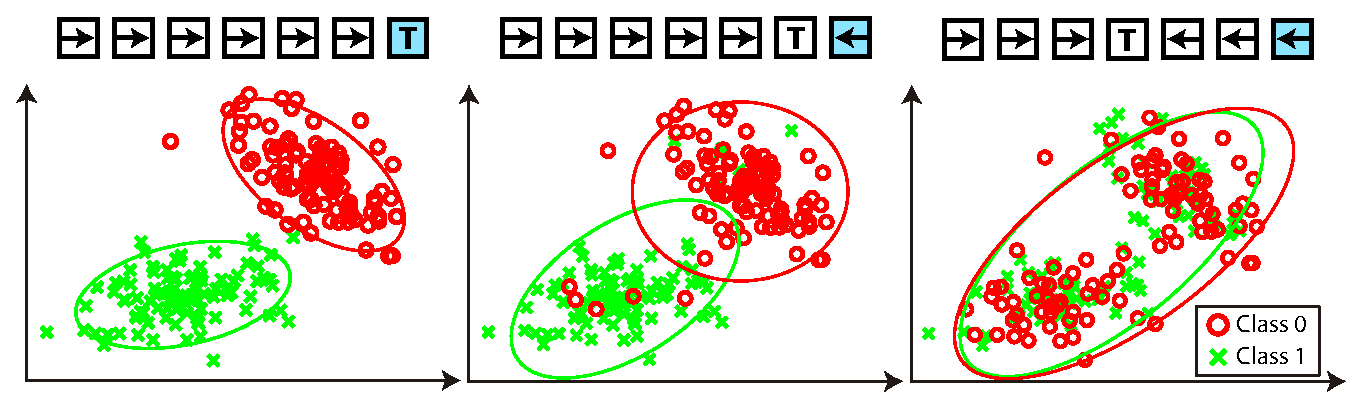
\includegraphics[width=\columnwidth]{img/real_vs_fake.eps}
%\caption{Hypothesis label spaces for a 1D grid world. For the represented example, the arrows indicate for each state what action should elicit a positive feedback to reach the state marked with T (i.e., the optimal policies). Below are shown the received signals (represented as points in a 2D feature space) labeled according to their respective task hypothesis. Corresponding 2D Gaussian distributions estimates are overlaid. While for the correct target (shaded blue state) the distributions shows a large separability (Left), the overlaps increases as the believed target moves away from the real one (Middle, Right).}
%\label{fig:intuition}
%\end{figure}
%



% Perceptual learning and task learning can both benefit from user interaction in many different ways. On the one hand, if the interaction protocol and context, is well defined it is possible to acquired grounded perceptual data. On the other hand, if the human and the machine understand each others, the human can explain or guide the machine, which may reduce learning time or even enable the machine to learn task difficult to write down as an objective or reward function.


% Machine-learning and artificial intelligence research aims at giving computers the ability to learn without being explicitly told. Two widely explored subfields are perceptual learning, in which the system learns to discriminate between perceptual events, and task learning, in which the system learn to increase its performance wrt. an objective or a reward function. 
% Well known results include hand writing recognition \todo{cite}, scene analysis \todo{cite} on the perceptual learning side and \todo{stuff} on the task learning side.

% For long most of the task learning research focused on abstract, well structure, problems. More recently, machine and in particular machines, are \todo{believed to be useful in our daily life}. Such machine will need the ability to learn new task in open-ended environment were an objective or reward function is not easy to define. Current approaches consist of inferring the reward function by interacting with others (e.g. humans) who already acquired the skill. \todo{This field is known as learning from demonstration. Inverse Reinforcement Learning is.}

% However most of those systems have not considered in depth the properties of teaching interactions with a human in the loop. This issues have began to be addressed in works studying interactive learning \todo{cite}, which combines the ideas of learning from demonstration, learning by exploration and tutor feedback.

% Recently interactive learning as acquired increasing attention.

%Under this approach, the teacher interacts with the machine and provides extra feedback or guidance. In addition, the machine can act to improve its learning efficiency. Recent developments have considered: extra reinforcement signals \todo{cite}, action requests \todo{cite}, disambiguation among actions \todo{cite}, preferences among states \todo{cite}, iterations between practice and user feedback sessions \todo{cite} and choosing actions that maximise the user feedback \todo{cite}.

% Perceptual learning and task learning can both benefit from user interaction in many different ways. On the one hand, if the interaction protocol and context, is well defined it is possible to acquired grounded perceptual data. On the other hand, if the human and the machine understand each others, the human can explain or guide the machine, which may reduce learning time or even enable the machine to learn task difficult to write down as an objective or reward function.

% While impressive results have been obtained in each domain, 
% However most work considered them separately:
% \begin{itemize} 
% \item In perceptual learning from human interaction perceptual events are learned to be categorized. The human provides signals related to some perceptual events. Associating perception and human signals implies \textbf{the machine is aware of the communicative goal of the human}.
% associated to their respective names.
% human 's communicative signals are learn to be associated to their respective meanings. 
% Such learning often rely on supervised classification methods, which implies collecting data samples associated with their respective names (called labels), which are provided by the human partners. This latter requirement implies \textbf{the machine is aware of the communicative goal of the human}.
% \item In task learning from human interaction most work has focused on how to extract statistical task models from human teaching signals. Therefore a usual assumption is that \textbf{the machine understands the meanings of human' s  communicative signals}.
% \end{itemize}


% The system is updating as many models as task hypothesis and is looking for the one from which emerges a coherence in the prediction of the user signals by the classifier and the expected meanings from the hypothesis.


% \todo{In machine learning terms, given the dataset of signals $e$, the best set of labels is the one producing the classifier of best accuracy. In other words, we will select the set which display a more coherent structure between the labels and the spacial organization of signals, according to the assumptions, constraints and biases of the classification algorithm used.}

% An intuition on how the algorithm works is to imagine the agent assigning hypothetic labels (i.e. meanings) to signals for each possible task. The system is updating as many models as task hypothesis and is looking for the one from which emerges a coherence in the prediction of the user signals by the classifier and the expected meanings from the hypothesis.


% An important consequence of this algorithm is that once a first task has been identified correctly, the true label of the received signals are known. Hence, once a first task has been learnt from scratch, it becomes equivalent to a calibration procedure, and the next task to be learn will be similar to a task learning problem from known signal to meaning mapping learnt from a calibration procedure. \todo{it is even improved}






% We call this problem learning from unlabelled interaction frame or joint perceptual and task learning.
%
% Frames are a concept that emerges simultaneously in social theory \cite{goffman1974frame} and artificial intelligence \cite{minsky1974framework}. They represents a stereotyped situations, a schema of interpretation given a particular situation or event. It is answering the question: \emph{what is going on here ?},  in order to reduce ambiguity of intangible topics by contextualizing the information.
%
% Interaction frames are the subclass of frames that account for interaction scenario. A simple interaction frame would be a human providing discrete action advice to a machine in the context of a reaching task. Being aware of this frame, the machine knows the utterances of the user correspond to action it should perform to achieve user intended goal. In task learning, such frame is often assumed to be known by both the human and the machine in addition to the signal-to-meaning classifier that translate the actual user signal into meaningful symbols.
%
%A simple interaction frame would be a human presenting an object to a machine at the same time as saying the name of the object. Being aware of this frame, the machine knows the utterance correspond to the name of the object (and not its shape or color). In others words the label of the speech signal is given.
%
% An unlabelled interaction frames correspond to a loosely defined interaction frame in which the interactive partners knows what kind of signal to expect but not the particular details of it. Following our example, a loosely defined frame would be cases where the signal-to-meaning classifier is unknown to the machine. What remains is the fact the interaction is constrained, and the user is known to deliver signal that correspond to desired action from the machine in order to achieve a task. In other word the label of the unknown speech signal is not explicitly given but is known to belong to one of a finite set of possible meanings.
%the human saying either the name, the color or the shape of the object.
%
% Such unlabelled interaction frame is at the core of our approach, it is assumed to be known by both the human and the machine in order for our algorithm to work. It includes both the context in which the interaction in taking place, e.g. teaching a machine which state to reach in the world, and the protocol used by the teacher to communicate to the machine, e.g. the teacher assessing machine's action.

% The problem we want to solve resumes in trying to learn what to do without knowing what we are told to do. 

%!TEX root = aaai2014.tex
\section{ALGORITHM}
\label{sec:algorithm}

\subsection{Problem definition}

We consider interaction sessions where a machine can perform discrete actions from a set of available actions $a \in \mathcal{A}$ in an either discrete or continuous state space $s \in \mathcal{S}$. The user, that wants to achieve a task $\hat{\xi}$, is providing feedback to the machine using some specific signal $e$, represented as a feature vector. The task is sequential meaning it is completed by performing a sequence of actions. The machine ignores the task the user has in mind, as well as the actual meaning of each user's signal. Its objective is to simultaneously solve the task and learn a model for the user's signals. To achieve this, it has access to a sequence of triplets in the form $D_M = \{(s_i, a_i, e_i),\ i = 1,\ldots,M\}$, where $s_i$, $a_i$ and $e_i$ represent, respectively, the state, action and instruction signals at time step $i$. The behavior of the machine is determined by the actions $a\in\mathcal{A}$ and the corresponding transition model $p(s'\mid s,a)$.


We make the following assumptions under this general paradigm. First, the system has access to a set of tasks $\xi_1,\ldots,\xi_T$ which includes the task the user wants to solve. We assume the instruction signals $e$ have a finite and discrete number of meanings $l \in \{l_1, l_2, \ldots, l_L\}$ which we call labels and this is known by the user and the machine. In this work we will consider two possible meanings for the signals: correct or incorrect; but more complex meanings could be used, such as guidance instructions (go up, go left, ...). We assume that given these labels, it is possible to compute a model that generates or classifies signals $e$ into meanings $l$. The parameters of such a model will be denoted by $\theta$ and we assume this mapping between signal $e$ and their label $l$ to be fixed. However this mapping is unknown to the agent at start.


%The meaning of  model is unknown at start and is parametrize by $\theta$. Given a label $l$ it outputs the probability that an observed signal $e \in \mathbf{R}^n$ was generated by our model $p(e | l, \theta)$.
 
% the signal-to-meaning mapping. This mapping is done by a classifier parameterize by $\theta$, that is unknown at start. Given a signal $e \in \mathbf{R}^n$ the classifier outputs label probabilities $p(l^{H^\theta} | e, \theta)$.

%We further assume that given a task $\xi$ and a state-action pair $(s, a)$, the machine has access to a model of the user expected labels $p(l^{H} | s, a, \xi)$. We denote as $D_i^\xi$ the history of $(e_i, s_i, a_i, p(l_i^{H} | s_i, a_i, \xi))$ up to time $i$ for task $\xi$. 
%Given $D_i^\xi$, we can optimize the classifier parameters $\theta_i^{\xi}$.


% For each hypothesis, at time $i$, we have several dataset $D_i^{\xi_t}$, which are used to train a classifier parametrize by $\theta_i^{\xi_t}$. Each classifier $\theta_i^{\xi_t}$ represents an interpretation hypothesis of the user given he is trying to instruct the task $\xi_t$.

\subsection{Estimating Tasks Likelihoods}

% \todo{Conceptual terms, no Gaussian classifier, no EEG}

We start by assuming we are provided a signal decoder $\hat{\theta}$ and relax this assumption later on.
%
As mentioned in the introduction, knowing $\hat{\theta}$, we can compute the probability of each task $\xi_t$ after observation of a signal $e$ when performing action $a$ in state $s$:
%
\begin{eqnarray}
p(\xi_t|e, s, a, \hat{\theta}) & \propto & p(e |s, a, \hat{\theta}, \xi_t) p(\xi_t)
\label{eq:1}
\end{eqnarray}
%
where  $p(e |s, a, \hat{\theta}, \xi_t)$ needs to take into account the probability of each possible meaning $l$ given the target $\xi_t$, the current state $s$ and the action $a$ executed by the machine:
%
\begin{eqnarray}
p(e |s, a, \hat{\theta}, \xi_t) =  \sum_{k \in {1, \ldots, L}} p(e |l = l_k, \hat{\theta}) p(l = l_k| s, a, \xi_t)
\end{eqnarray}

This process can be repeated recursively for several interaction steps $i$:
%
\begin{eqnarray}
\L_i^{\xi_t} & = & p(\xi_t|D_i^{\xi_t}, \hat{\theta}) \nonumber \\
& \propto & p(e_i |s_i, a_i, \hat{\theta},\xi_t) p(\xi_t|D_{i-1}^{\xi_t}, \hat{\theta})
\label{eq:filter}
\end{eqnarray}
%
with $p(\xi_t|D_0^{\xi_t}, \hat{\theta})$ being the prior at time 0 (before the experiment starts) for the task $\xi_t$, usually uniform over the task distribution. 

% Also, if we knew what task the user had in mind at every time step ($\xi_{1:i}$), one could estimate $p(\theta \mid D_i, \xi_{1:i})$, that is, the posterior distribution of the meaning parameters given the task being solved at each point in time. Note the different notation for the task and the meaning parameters. The reason is that $\theta$ is a shared parameter for different tasks, while the task being solved should in principle not affect the meaning of the signals $e$.

%By normalizing the likelihoods of all task, we obtain the probability distribution between tasks. A threshold mechanism could be used to decide when to stop.

We now relax the assumption we are given a model $\hat{\theta}$. The natural extension from the previous models is to compute the posterior distribution over the task and the model, $p(\xi, \theta |e, s, a)$. However, the resulting distribution does not have a close form solution even when linear Gaussian likelihoods are used due to the combination of mixtures for each possible task. Another alternative is to compute the $\theta$ and $\xi$ that maximize the data likelihood. This is prone to fail in certain scenarios due to two reasons. First, it is common that different tasks share many labels (e.g. the policies to reach neighboring cells on a grid world are almost identical and, therefore, share most of the labels $l$) and results on large uncertainties in the task space that require multiple actions to be disambiguated. Second, if the signals are not well separated the meaning parameters $\theta$ of different tasks will not differ much.  

For instance, under Gaussian assumptions for $p(e |l = l_k, \theta)$ and deterministic task labels $p(l = l_k| s, a, \xi)$, it is possible to integrate out  $\theta$ to compute the marginal likelihood $p(D_M\mid \xi)$. The resulting likelihood depends only on the traces of each $p(e |l = l_k, \theta)$. Empirical results with synthetic and EEG data for a reaching task on a grid revealed that, when the distributions over $e$ overlap, the traces were not enough to recover the most likely task and the corresponding meaning parameters. 

To cope with these problems, we define the following pseudo-likelihood function:
%
\begin{eqnarray}\label{eq:pseudo1}
\lefteqn{P(D_M | \xi, \theta) \approx \prod_{i=1}^M p(e_i | s_i, a_i, \xi, \theta_{-i})}  \\ \label{eq:pseudo2}
&=& \prod_{i=1}^M \sum_{l_c}\sum_l  p(e_i | l_c, \theta_{-i})  p(l_c | l, \theta_{-i}) p(l|s_i,a_i,\xi)
%p(\xi_t, \theta^{\xi_t} |e, s, a) & \propto & p(e | s, a, \xi_t, \theta^{\xi_t}) p(\xi_t, \theta^{\xi_t}).
\label{eq:}
\end{eqnarray}
%
where $l$ represents the meaning assigned by task $\xi$, action $a_i$ and state $s_i$ and $l_c$ is the label corrected based on what we know about our classifier $\theta_{-i}$ for a given label $l$.

The pseudo-likelihood is built using a leave-one-out cross-validation strategy to evaluate the likelihood $p(e_i | s_i, a_i, \xi, \theta_{-i})$ of each signal based on the meaning parameters $\theta_{-i}$ learned for each task using all the other available signals. The use of $\theta_{-i}$ indicates we use a leave one out method. If we interpret $p(e_i | s_i,a_i,\xi,\theta_{-i})$ as a classifier, its predicted labels should match the ones provided by the task for different state-actions pairs. The rationale behind it is that for the correct task, the signals and labels will be more coherent than for other tasks, which we measure as the predictive ability of a classifier trained on the signal-label pairs. Note that wrong tasks will assign wrong labels $l$ to the signals $e$, therefore the learned models will have larger overlaps (see Figure~\ref{fig:planningExplained}c). 

% resulting in higher likelihoods. Coherence between signals and labels is measured as the predictive ability of a classifier trained on the signal-label pairs. The use of $\theta_{-i}$ indicates we use a leave one out method. If we interpret $p(e_i | \xi, \theta_{-i},s_i,a_i)$ as a classifier, its predicted labels should match the ones provided by the task for different state-actions pairs. Note that wrong tasks will assign wrong labels $l$ to the signals $e$ and, therefore, the learned models will have larger overlaps. See the discussio of Figure~\ref{fig:planningExplained}. 

Each term of the pseudo-likelihood is computed from three terms. $p(l|s_i,a_i,\xi)$ represents the probability distributions of the meanings according to a task, the executed action and the current state.   $p(l_c | l, \theta_{-i})$ encodes which label will be actually recovered by $\theta_{-i}$. Intuitively, it models the quality of the model $\theta_{-i}$. $p(e_i | l_c,\theta_{-i})$ is the likelihood of the signal given the meaning. 
%
The pseudo-likelihood is maximized in two steps. First, the maximum a posteriori estimate $\theta_{-i}$ of each task is computed. Then, the term $p(l_c | l, \theta_{-i})$ is approximated by the corresponding confusion matrix of the classifier based on $\theta_{-i}$. It is the probability that the classifier itself is reliable in its prediction. Finally, the best task $\xi$ should be the one that maximizes the pseudo-likelihood in Eq. \ref{eq:pseudo1}.

%
%A sensible option is to perform independant update of classifier and task. For each task, at time $i$, we have a dataset $D_i^{\xi_t}$, which can be used to train a classifier parametrize by $\theta_i^{\xi_t}$. Each classifier represents an interpretation hypothesis of the user signals given he is instructing the task $\xi_t$.
%
%Incorporating $\theta_i^{\xi_t}$ in equation \ref{eq:filter} we obtain:
%
%\begin{eqnarray}
%\L_i^{\xi_t} & = & p(\xi_t|D_i^{\xi_t}, \theta_i^{\xi_t}) \nonumber \\
%& \propto & p(e_i |s_i, a_i, \theta_i^{\xi_t}, \xi_t) p(\xi_t|D_{i-1}^{\xi_t}, \theta_{i-1}^{\xi_t})
%\label{eq:filter}
%\end{eqnarray}
%with $p(\xi_t|D_0^{\xi_t}) = \frac{1}{T}$.
%
%\todo{no $p(\theta)$, it is not good, maybe
%\begin{eqnarray}
%\L_i^{\xi_t} & = & \int_{\theta_i^{\xi_t}} p(\xi_t|D_i^{\xi_t}, \theta_i^{\xi_t}) p(\theta_i^{\xi_t}) d\theta_i^{\xi_t} \nonumber \\
%\label{eq:filter}
%\end{eqnarray}
%}
%
%Unfortunatly as the models used to evaluate the new evidences are different for each task hypothesis we can not compare directly the likelihoods by simply normalizing them.
%
%
%In order to weight appropriatly the estimates, we would like to known if the prediction of our model can be trusted \todo{this shouldn't be $p(\theta)$ in the model above?}. As we do not have access to the true repartition of signal or the true model we must rely on other empricial metric. Our hypothesisis is that for the correct task the system will associated the correct label. The resulting dataset should be more separable than the others who will mix the labels (see figure \ref{fig:planningExplained}c). To estimate this separability, we compute the classification performance of our model on the labeled data. Our system is looking for the hypothesis from which emerges a coherence between the spacial organization of label in the feature space and their associated labels.
%
%Hence we define a new metric in the label space. We will compare the expected user labels $p(l^{\xi_t} | s, a, \xi_t)$ with the labels intended by the user $p(l^{\theta} | e, \theta)$. The more the predictions match, the more likely the task. By using this estimate we can include a performance measure on the classifier prediction $p(l^{\theta} | e, \theta)$ by relying a cross validation procedure. \todo{maybe we can explain other approcahes, like estimating the overlap of the two distributions}
%
%We can compute the probability:
%\begin{eqnarray}
%J^{\xi_t}(e,s,a) & = & \sum_{k \in {1, \ldots, L}}  p(l^{\xi_t} = k | s, a, \xi_t) p(l^{\theta^{\xi_t}} = k | e, \theta^{\xi_t}) \nonumber \\
%\end{eqnarray}
%With $p(l^{\theta^{\xi_t}} = k | e, \theta^{\xi_t})$ computed via a cross validation procedure. \todo{it mean that there is several $\theta$ used here, maybe replacing them with $D_i^{\xi_t}$}
%
%\todo{At each new step, we can compute the likelihood of each task by cumulating the evidence.}
%
%\begin{eqnarray}
%\L^{\xi_t} = \prod_{i \in {1, \ldots, M}} J^{\xi_t}(e_i,s_i,a_i)
%\end{eqnarray}

\subsection{Decision and Task Change}

% The machine is simultaneously solving a task and learning the meanings associated to the signals. However, it is possible to solve the task before the meanings are perfectly modeled or vice-versa. Therefore, in practical terms it is necessary to be able to switch to the next task once it has been solved and to continue updating the meaning. 

The machine must decide which task is the correct one. To do so, we define $W^{\xi_t}$ the minimum of pairwise normalized likelihood between hypothesis $\xi_t$ and each other hypothesis: 
%
\begin{eqnarray}
W^{\xi_t} = \min_{x~\in~{1, \ldots, T} \smallsetminus \{t\}} \frac{P(D_M | \xi_t, \theta)}{P(D_M | \xi_t, \theta) + P(D_M | \xi_x, \theta)}
\label{eq:weight}
\end{eqnarray}

When it exists a $t$ such that $W^{\xi_t}$ exceeds a threshold $\beta \in ]0.5,1]$ we consider task $\xi_t$ is the one taught by the user.

Once a task is identified with confidence, the robot executes it and prepares to receive instructions from the user to execute a new task. Assuming the user starts teaching a new task using the same kind of signals, we now have much more information about the signal model. Indeed, we are confident that the user was providing instructions related to the previously identified task; therefore we can infer the true labels of the past signals. We can now  assign such labels to all hypothesis and by using the same algorithm we can start learning the new task faster as all hypothesis now share a common set of signal-label pairs. The meaning models for each hypothesis are still updated step after step until the new task is identified and labels reassigned.

%%%%%%%%%%%%%%%%%%%%%%%%%%%%%%%%%%%%%%%
%%%%%%%%%%%%%%%%%%%%%%%%%%%%%%%%%%%%%%%
%%%%%%%%%%%%%%%%%%%%%%%%%%%%%%%%%%%%%%%
%%%%%%%%%%%%%%%%%%%%%%%%%%%%%%%%%%%%%%%
%%%%%%%%%%%%%%%%%%%%%%%%%%%%%%%%%%%%%%%
%%%%%%%%%%%%%%%%%%%%%%%%%%%%%%%%%%%%%%%
%%%%%%%%%%%%%%%%%%%%%%%%%%%%%%%%%%%%%%%
%%%%%%%%%%%%%%%%%%%%%%%%%%%%%%%%%%%%%%%
%%%%%%%%%%%%%%%%%%%%%%%%%%%%%%%%%%%%%%%
%%%%%%%%%%%%%%%%%%%%%%%%%%%%%%%%%%%%%%%
%%%%%%%%%%%%%%%%%%%%%%%%%%%%%%%%%%%%%%%
%%%%%%%%%%%%%%%%%%%%%%%%%%%%%%%%%%%%%%%
%%%%%%%%%%%%%%%%%%%%%%%%%%%%%%%%%%%%%%%
%%%%%%%%%%%%%%%%%%%%%%%%%%%%%%%%%%%%%%%
%%%%%%%%%%%%%%%%%%%%%%%%%%%%%%%%%%%%%%%
%%%%%%%%%%%%%%%%%%%%%%%%%%%%%%%%%%%%%%%
\begin{comment}

At next time step $i+1$ we can compute the probability:
\begin{flalign}
& J_{i+1}^{\xi_t}(s_{i+1},a_{i+1},e_{i+1}) = \nonumber \\
& = \sum_{l \in {1, \ldots, L}} p(l_{i+1}^{H^{\xi_t}} = l \cap l_{i+1}^{H^{\theta_{i}^{\xi_t}}} = l | e_{i+1}, s_{i+1}, a_{i+1}, \xi_t, \theta_{i}^{\xi_t}) \nonumber \\
& = \sum_{l \in {1, \ldots, L}}  p(l_{i+1}^{H^{\xi_t}} =l | s_{i+1}, a_{i+1}, \xi_t) p(l_{i+1}^{H^{\theta_i^{\xi_t}}} = l | e_{i+1}, \theta_i^{\xi_t})
\end{flalign}
given a classifier $\theta_i^{\xi_t}$ trained on past interaction $D_i^{\xi_t}$. As the classifier changes every step, equation \ref{eq:joint} becomes recursive:

\begin{eqnarray}
\L_{i+1}^{\xi_t} =   %\L_{i}^{\xi_t} \sum_{l \in {1, \ldots, L}} p(l_{i+1}^{\xi_t} = l\cap l_{i+1}^{\theta_i^{\xi_t}} = l | e_{i+1}, s_{i+1}, a_{i+1}, \xi_t, \theta_i^{\xi_t}) \nonumber \\
%& = &
J_{i+1}^{\xi_t}(s,a,e)~~\L_{i}^{\xi_t} 
 % \sum_{l \in {1, \ldots, L}} p(l_{i+1}^{H^{\xi_t}} =l | s_{i+1}, a_{i+1}, \xi_t) \ldots \nonumber \\
% \ldots p(l_{i+1}^{H^{\theta_i^{\xi_t}}} = l | e_{i+1}, \theta_i^{\xi_t})
\label{eq:algo}
\end{eqnarray}
with $\forall t, \L_{0}^{\xi_t} = 1$.

\textbf{Why would it works?} Because the user is behaving only according to one task hypothesis and the coherence between spacial organization of signals and their associated labels should be higher for the correct hypothesis, see figure \ref{fig:intuition}. The chosen classifier --- by its assumptions, constraints and biases --- indirectly measure this coherence by making inconsistent predictions. Accounting for such uncertainty in predictions is primordial for our algorithm to work.

\subsection{Modeling Classifier Uncertainty}

At every time step, we empirically model the uncertainty of our classifiers predictions by estimating their associated confusion matrix. We use a 10 fold cross validation procedure on the training data $D_i^{\xi_t}$. The confusion matrix gives us the probability that the true label was $i$ given our classifier prediction was $j$. It is used to temperate the predictions $p(l_{i+1}^{H^{\theta_i^{\xi_t}}} = l | e_{i+1}, \theta_i^{\xi_t})$ which decomposes as:

\begin{eqnarray}
\sum_{k = 1,\ldots, L} p(l_{i+1}^{H^{\theta_i^{\xi_t}}} = l| l_{i+1}^{\theta_i^{\xi_t}} = k) p(l_{i+1}^{\theta_i^{\xi_t}} = k | e_{i+1}, \theta_i^{\xi_t})
\label{eq:conf}
\end{eqnarray}
with $p(l_{i+1}^{\theta_i^{\xi_t}} = k | e_{i+1}, \theta_i^{\xi_t})$ the raw output of the classifier and $p(l_{i+1}^{H^{\theta_i^{\xi_t}}} = l| l_{i+1}^{\theta_i^{\xi_t}} = k)$ given by the confusion matrix 

\subsection{Decision}

We define $W^{\xi_t}$ the minimum of pairwise normalized likelihood between hypothesis $\xi_t$ and each other hypothesis:

\begin{eqnarray}
W^{\xi_t} = \argmin_{x~\in~{1, \ldots, T} \smallsetminus \{t\}} \frac{\L^{\xi_t}}{\L^{\xi_t} + \L^{\xi_x}}
\label{eq:weight}
\end{eqnarray}

When there exists a $t$ such that $W(\xi_t)$ exceed a threshold $\beta \in ]0.5,1]$ we consider task $\xi_t$ is the one taught by the user.

\subsection{From Task 1 to Task 2}

After identifying a first task, we can infer the true labels of the past data and assign such labels for all hypothesis. At this iteration only, all hypothesis have a similar classifier. The user starts teaching a new task using the same kind of signals. By using the same algorithm we can start learning this new task faster as all hypothesis share a common set of signal-label pairs. The classifier keeps being updated step after step until next task is identified and labels reassigned.

\end{comment}



% %!TEX root = aaai2014.tex
\section{Implementation}
\subsection{Task}

We have a 5x5 grid world modeled as a MDP, with known Transisiton proba. Non stochastic transition.
One task is defined as a reward of one in one state. There is 25 states, hence 25 task hypothesis.
The optimal policy, that the user is supposed to use as reference, is computed using Value Iteration by acting greedy on the Q-Values.

\subsection{Expected label}
\begin{equation*}
    p(l^\xi | s, a, \xi) = 
    \begin{cases}
	1-\alpha               & if~a = \argmax_a \pi^{\xi}(s,a)\\
        \alpha             & \text{otherwise}\\
   \end{cases}
\end{equation*}
with $\alpha$ modeling the expected error rate of the user. I am using an alpha of $0.1$.

\subsection{Classifier}
\subsubsection{Training}

One mean and covariance per class. I compute the weighted mean and weighted covariance for each label using $p(l^\xi | s, a, \xi)$ as weights. I then apply skrinkage to the covariance, I use an $\lambda = 0.5$.

\textbf{What can be discussed:} \\
\\
Weighted mean: $\bar{x}^* = \frac{\sum_{i=1}^n w_i x_i}{\sum_{i=1}^n w_i}$
\\
\\
Weighted covariance: I use $\sum w_i (x - \bar{x}^*)^T  (x - \bar{x}^*) / \sum w_i$. This is a biased estimation. It may be better to divide by $\sum w_i - 1$ which is called Bessel correction. Actually it seems there is an other version for the factor $\frac{\sum_{i=1}^n w_i}{(\sum_{i=1}^n w_i)^2-(\sum_{i=1}^n {w_i^2})}$ which seems to be more suited. I do not think this is important.
\\
\\
Shrinkage: $regCov = (1 - lambda) * cov + (lambda / length(cov)) * trace(cov) * eye(size(cov))$

\subsubsection{Testing}

For one signal $e$, I compute the value of the marginal pdf function using the non-informative prior for each labels $z$: $p(e|\theta, l=z) = \int p(e|\theta, l=z) d\theta$.

The integral above is the following equation, I took it from murphy technical notes and tested my implementation on various test bench:
\begin{eqnarray}
p(e|\theta) = t_{n-d}(e | \bar{x}, \frac{S (n+1)}{n(n-d)})
\end{eqnarray}
where for a given class $z$:\\
\begin{itemize}
\item $n$ is the number of point in $x$
\item $d$ is the dimensionality of the data
\item $x$ is the data I use to train, $\bar{x}$ is the mean. I use the weigthed mean here.
\item $S = \sum_{i} (x_i - \bar{x}) (x_i - \bar{x})^T$ is the covariance. I use the weigthed covariance here.
\end{itemize}
This can only be computed after d+1 step, i.e. 35 points in our EEG case.

\textbf{What can be discussed:} As I am computing the weighted mean and covariance, $n$ is hard to define. If I was using non-weighted labels, then I could only start computing things after at least 70 iterations. And this is only in the best case, in reality we have many hypothesis with different labeling, it is more probable we would need at least 100 points to start using the classifiers. I am using $n$ equal to the number of steps. 


Finally to compute $p(l = j | e, \theta) = \frac{p(e|\theta, l=j)}{\sum_z p(e|\theta, l=z)}$

\subsubsection{Correcting}

The prediction of the classifer may be wrong, the fact the classifier output probabilistic label is not a solution to this problem. If it predict 100\% one label is can still be wrong. We model this using the confusion matrix. I am using a probabilistic version of the confusion matrix (which reduces to counting true positive, true negative, \ldots if non-proabilisitc label and prediction).

\begin{eqnarray}
Conf(i,j) &=& \frac{\sum_{k \in 1:N} p(l_k = i \cap l = j| s_k, a_k, \xi, e_k, \theta)}{N} \nonumber \\
&=& \frac{\sum_{k \in 1:N} p(l_k = i| s_k, a_k, \xi) p(l = j| e_k, \theta)}{N} \nonumber \\
\end{eqnarray}
with $p(l_k = i| s_k, a_k, \xi)$ the labels used to train, and $p(l = j| e, \theta)$ the label predicted from the classifier.

I am estimating the confusion matrix via a 10 folds cross validation procedure.

\textbf{What can be discussed:} Why not a ``hard'' confusion matrix, i.e.\ counting the number of true positive, true negative, \ldots ? The probabilisitic is more precise. For ``hard'' confusion matrix, consider the case of one classifier that always output 51/49 or 49/51 percent proba but is always as correct the ``hard'' way than an other that is 99/1 or 1/99 percent. It depends on the context, in ours we prefer a probabilisitic version of the confusion matrix which will differentiate such cases.

From the confusion matrix, we can compute the corrected probability of one label given the probability outputted by the classifier.

\begin{eqnarray}
p(l = i | l^\theta = j)  = \frac{Conf(i,j)}{\sum_i Conf(i,j)} \nonumber \\
\end{eqnarray}

In practise it is easier to directly normalize the confusion matrix per column, i.e. column sums to one.

\subsection{Algo}


\begin{enumerate}
\item perform action $a$ in state $s$
\item collect signal $e$
\item for each hypothesis $\xi$, assign label $p(l^\xi | s, a, \xi)$.
\item for each hypothesis $\xi$, train a classifier $\theta^\xi$
\item for each  hypothesis $\L(\xi) = 1$
\item repeat from step 1 until ready to compute stuff
\item perform action $a$ in state $s$
\item collect signal $e$
\item for each hypothesis $\xi$, assign label $p(l^\xi | s, a, \xi)$.
\item for each hypothesis $\xi$, use previously trained classifier to estimate $p(l^{\theta^\xi} | e, \theta^\xi)$
\item for each hypothesis $\xi$, correct $p(l^{\theta^\xi} | e, \theta^\xi)$ with the confusion matrix. for each i, correct $p(l = i | l^\theta) = \sum_{j} p(l = i | l^\theta = j) p(l^\theta = j)$ with  $p(l = i | l^\theta = j) = \frac{Conf(i,j)}{\sum_i Conf(i,j)}$, we call the corrected label $p(l^U | e, \theta^\xi)$
\item update each hypothesis likelihood by the joint probability that predicted label equal expected label: $\L^\xi = \L^\xi * \sum_l p(l^\xi = l | s,a,\xi) p(l^U = l| e, \theta^\xi)$.
\item for each hypothesis $\xi$, train a new classifier $\theta^\xi$ including all data
\item go to step 7
\end{enumerate}


\subsection{Stopping criterion}

I changed the stopping criterion. We want the best hypothesis to be X times more likely than all the other. In other word the min of the likelihood ratio should be above a threshold. I am using a threshold of 0.9.

\begin{eqnarray}
\argmin_{t~\in~T \smallsetminus \{x\}} \frac{\L^{\xi_x}}{\L^{\xi_t}}
\end{eqnarray}

\textbf{What can be discussed:} Why not normalizing likelihoods ? Consider two cases: a) two hypothesis only, likelihoods are [0.45, 0.05], normalized likelihood is [0.9,0.1], min likelihood ratio [0.9, 0.111]; b) four hypothesis [0.45, 0.05, 0.05, 0.05], normalized likelihoods are [0.75, 0.083, 0.0833, 0.083], min likelihood ratio [0.9, 0.111, 0.111, 0.111]. Scale it to 1000 hypothesis and the normalized likelihood takes huge amount of time to reach a specific threshold. Normalized likelihood would require to change the threshold for every scenario. The likelihood ratio solves this problem and make sure one hypothesis likelihood is X times more likely that all others on an individual bases.

\subsection{After confidence reached}

We plan greedy to the target. Then we assign all the past labels of the target hypothesis to all other hypothesis and start again. The classifier are now all the same which make the algorithm identical to one using only calibratoin, except that in our case step after step hypothesi classifiers will start to differ again. Which have nice effects on the number of error compared to fixed classifier.
%!TEX root = aaai2014.tex
\section{PLANNING UNDER UNCERTAINTY}
\label{sec:planning}

% After several interaction with the user, our algorithm is able to identify a task among a set of possible tasks. To do so it has to explore regions that allow to disambiguate among hypothesis. There are several efficient model-based reinforcement learning exploration methods that add an exploration bonus for states that might provide more learning gains. Several theoretical results show that these approaches allow to learn tasks efficiently \cite{brafman2003r,kolter2009near}. We define an uncertainty measure and use model-based planning to select sequences of actions that guide the agent toward states that better identify the desired task.

To solve our problem we need to identify simultaneously the task and how to interpret teaching signals. To do so the system has to explore regions that allow to disambiguate among hypothesis. There are several efficient model-based reinforcement learning exploration methods that add an exploration bonus for states that might provide more learning gains. Several theoretical results show that these approaches allow to learn tasks efficiently \cite{brafman2003r,kolter2009near}. We define an uncertainty measure and use model-based planning to select sequences of actions that guide the agent toward states that better identify the desired task.

In order to exemplify the specificity of our problem in terms of planning we present a simple experiment and compare the effect of different action selection strategies. In this scenario, the agent is in a T world with 7 states and can perform 4 actions (right, left, up, and down). The user wants the robot to reach the left edge (marked by G1) of the T, (see Figure~\ref{fig:planningExplained} top). The agent knows the users wants it to go to one of the two edges (G1 or G2) but not which one. The agent will perform some actions, and the user will assess the correctness of each agent's action by providing a two dimensional teaching signal. The agent does not known which signal means ``correct'' and which signal means ``incorrect''. As there is two possible tasks, the agent will assign labels to every user's signals according to each hypothesis. The result of the labeling process is displayed as colored dots (green for ``correct''and red for ``incorrect'') in Figure \ref{fig:planningExplained} (a, b, and c), where the left part corresponds to hypothesis 1 (G1) and the right part to hypothesis 2 (G2).

 % The goal of the agent is to reach one of the two edges of the T world (see figure \ref{fig:planningExplained} top), the one the user has in mind. After each agent's move, the user assesses the correctness of the agent action by providing a two dimensional teaching signal. 

\begin{figure}[!ht]
  \centering
      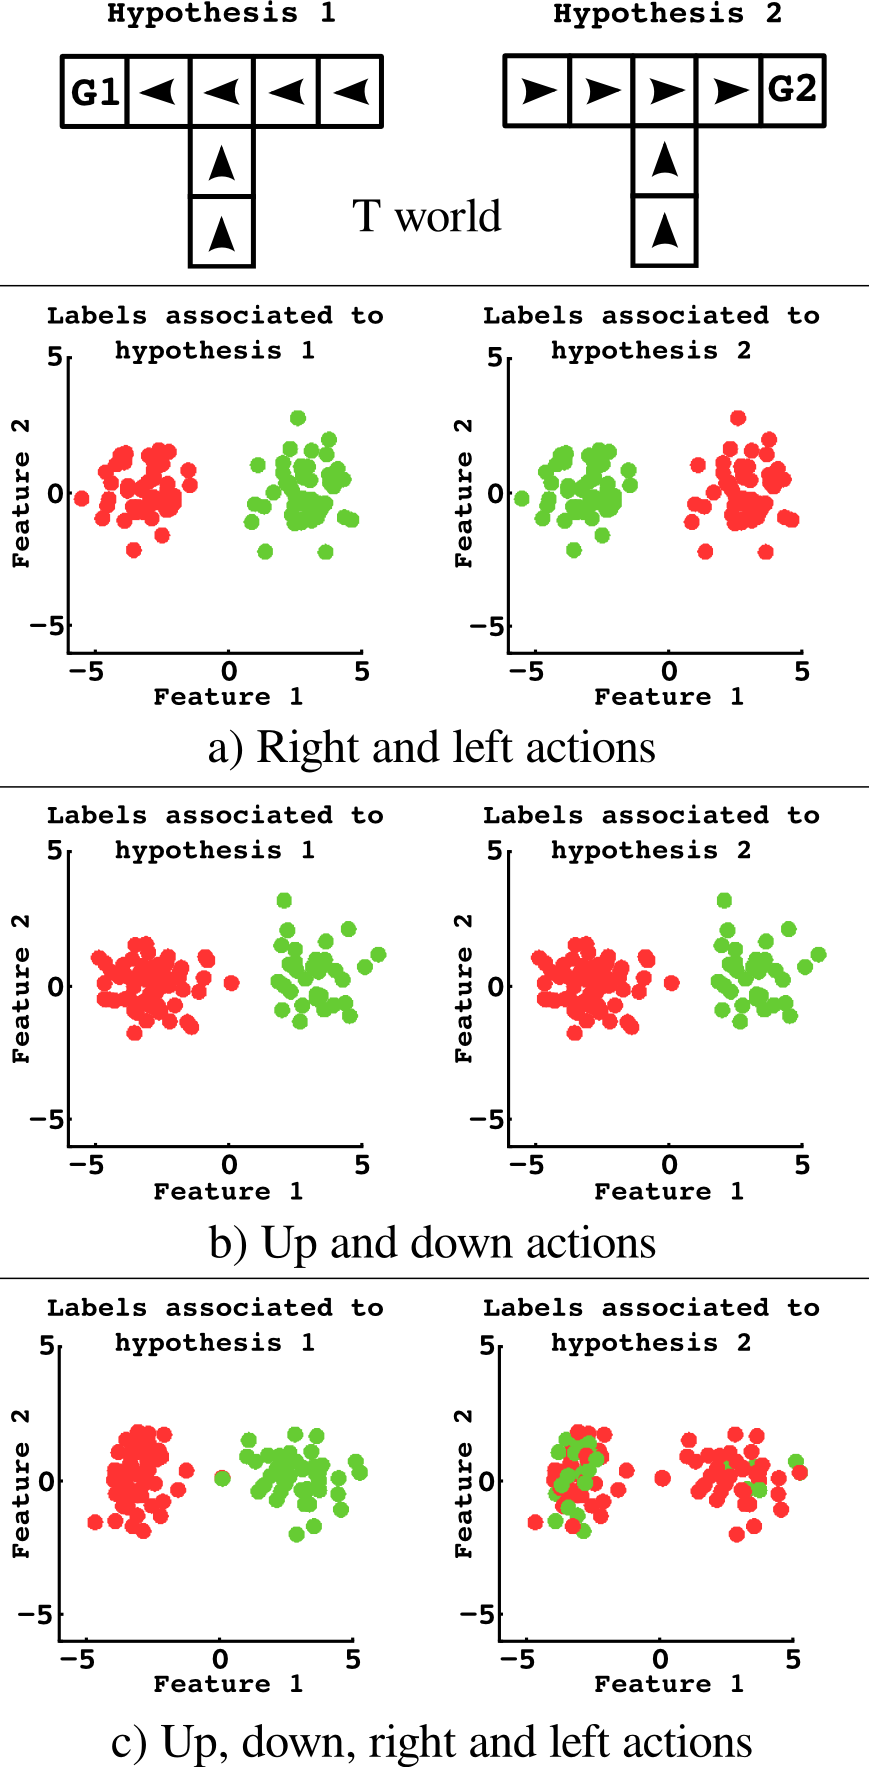
\includegraphics[width=0.93\columnwidth]{img/planning.png}
      \caption{A ``T world'' scenario and the interpretation results for different planning strategies. The agent knows it should reach either of the two edges of the T world (marked with the letter G). The arrows represent the optimal policy. For each move the agent receives an unlabeled two dimensional teaching signal, corresponding to user's assessments on the agent's actions. The teacher's goal is to have the agent reach G1. As the agent do not have access to this information, it interprets the signal according to each hypothesis (G1 and G2). a) shows the interpretation results if the agent only perform right and left actions in the top of the T world, b) shows the interpretation results when the agent only performs up and down actions in the trunk of the T, and c) shows the interpretation results for an agent performing all possible actions. Only the method c) allow to differentiate between hypothesis.}
    \label{fig:planningExplained}
\end{figure}

If the agent knew how to interpret the signal, i.e. which signal corresponds to correct or incorrect feedback, the optimal action to differentiate between the two hypothesis would be to perform right and left actions in the top part of the T. However in our problem the classifier is not given and the agent is building a different model for each hypothesis. As a results, we end up with two opposite interpretations of the user signal, which are both as valid (see Figure~\ref{fig:planningExplained}a) and do not allow to differentiate between hypothesis.

Considering that the agent does not know the signal to meaning classifier, a sensitive option is to select actions that allow to unequivocally identify the model. In our scenario taking only up and down actions in the trunk of the T leads to identical interpretation for each hypothesis (see Figure~\ref{fig:planningExplained}b). However this method do not allow to disambiguate between hypothesis and in most setting, such as the grid world we consider later, there is no state-action pair leading to unequivocal interpretations.

However performing all the four actions allow to disambiguate between hypothesis. As shown in Figure~\ref{fig:planningExplained}c, hypothesis 1 stands out by the nice coherence between the labels and the spacial organization of the data. This informs us that hypothesis 1 is the task the user has in mind and that feedback signals in the right and left part of the feature space means ``correct'' and ``incorrect'' respectively.

For our kind of problem the agent can not just try to differentiate hypothesis by finding state-action pair where expected feedback differs but should also collect data to build a good model or at least invalidate other models. Can we find a measure of uncertainty that account for both? Going back to Figure~\ref{fig:planningExplained} (a and b), we understand that, to differentiate hypothesis in situation a) the best actions to perform are up and down in the T trunk while in situation b) the best actions to perform are right and left in the top part of the T. This corresponds to the uncertainty in the signal space. In the case of a) when going left both hypothesis agree that they will receive a signal in the right part of the feature space even if they disagree on its meaning. However for action down, both hypothesis agree they should receive a signal of meaning ``incorrect'' but disagree on the expected location of such signal in the feature space. In the case of b) when going up both hypothesis agree they will receive a signal in the right part of the feature space and agree on its meaning. However for action left, both hypothesis disagree about the meaning of the signal they should receive and as both share the same signal model they expect a signal in different locations of the feature space.

Estimating uncertainty in the signal space is in practice too costly as it requires to compute, for every state-action pair, the overlap between many continuous probability distributions weighted by their respective expected contribution. Following the discussion presented in previous section, we will rely on our pseudo-likelihood metric. As we cannot predict, neither control, the signal we will receive for a particular state-action, we will rely on our past history of signal and compute the expected joint probability based on previously experienced signals.

% \todo{transition with actual equations, uncertainty in signal space is too costly to compute. We therefore rely on an approximation, projecting back signal space into some sort of expected meaning space and comparing with theoretical meaning space, i.e. the probability that expected labels $l^{H^{\xi_t}}$ equals predicted labels $l^{H^{\theta_{i}^{\xi_t}}}$}

% \todo{the following explanation was quite intuitive with respect to previous algo version but did not cover the details that I tried to explain above}

% To differentiate between tasks, our algorithm computes the probability that expected labels $l^{\xi_t}$ equals predicted labels $l^{\theta^{\xi_t}}$. In order to find which task is the correct one, we need to explore the state space where this value differs between likely hypothesis. As we cannot predict, neither control, the signal we will receive for a particular state-action, we will rely on our past history of signal and compute the expected joint probability based on previously experienced signals.

We note:
\begin{eqnarray}
J^{\xi_t}(s,a,e) = \sum_{l_c}\sum_l  p(e | l_c, \theta)  p(l_c | l, \theta) p(l|s,a,\xi_t) \nonumber
\end{eqnarray}
which is Eq.~\ref{eq:pseudo2} for only one new expected observation $e$, so the product over iterations disappears. And $J^{\xi}(s,a,e)$ the vector $[J^{\xi_1}(s,a,e), \ldots, J^{\xi_T}(s,a,e)]$.

The uncertainty of one state-action pair given a signal $e$ is computed as the weighted variance of the joint probability predictions with weights $W^{\xi} = [W^{\xi_1}, \ldots, W^{\xi_T}]$ (see Eq.~\ref{eq:weight}):
\begin{eqnarray}
U(s,a|e) = weightedVariance(J^{\xi}(s,a,e), W^{\xi})
\label{eq:planningOneSignal}
\end{eqnarray}

The uncertainty for a state-action pair is given by:
\begin{eqnarray}
U(s,a) & = & \int_{e} U(s,a|e) p(e) de
\end{eqnarray}
which we approximate by summing values of $U(s,a|e)$ for different signals $e$:
\begin{eqnarray}
U(s,a) & \approx & \sum_{e} U(s,a|e) p(e)
\label{eq:planning}
\end{eqnarray}
with $p(e)$ assumed uniform.
%

% Finally, we evaluate $U(s,a)$ by summing values of $U(s,a|e)$ for different signals $e$:
% \begin{eqnarray}
% U(s,a) & = & \int_{e} U(s,a|e) p(e) de \nonumber \\
% 		 & \propto & \sum_{e} U(s,a|e) p(e)
% \label{eq:planning}
% \end{eqnarray}

Our measure of global uncertainty $U(s,a)$ will be higher when, for a given state-action there is a high incongruity of expectation between each hypothesis and according to each hypothesis current probability. 

This measure is then used as a classical exploration bonus method. We will switch to a pure exploitation of the task after reaching the desired confidence level.

Interestingly this approach generalizes over other active sampling method \cite{lopes2009active}, if the classifier is known, equation \ref{eq:planningOneSignal} reduces to the one presented in \cite{macl11simul} and is no longer dependent on signal $e$. As our uncertainty function combines uncertainty on both signal and task space, when the former is known, the latter becomes the sole source of ambiguity.


% Our goal is to learn which task $\xi$ among a set of possible task $\xi_1,\ldots,\xi_T$ is the one taugh by the trainer. To do so we compute the cumulative probability that expected labels ($l_{i+1}^{\xi_t}$) equals predicted labels ($l_{i+1}^{U_t}$). In order to find which task is the correct one, we need to explore the space such that the expected joint probability between likely hypothesis differs.

% with weighted variance define as: \todo{cite if needed}
% \begin{eqnarray}
% wVar(x,w) = \frac{\sum_{i=1}^n w_i}{(\sum_{i=1}^n w_i)^2-(\sum_{i=1}^n {w_i^2})} \sum_{i=1}^N w_i \left(x_i - \bar{x}^*\right)^2
% \end{eqnarray}
% where: $\bar{x}^* = \frac{\sum_{i=1}^n w_i x_i}{\sum_{i=1}^n w_i}$

%Only the relative value of $U(s,a)$ matters and the use of variance is arbitrary, any function having similar properties of measuring variation between estimates would do.


% We note $J_{i}^{\xi}(s,a,e) = [J_{i}^{\xi_1}(s,a,e), \ldots, J_{i}^{\xi_T}(s,a,e)]$
%  % with:
% % \begin{eqnarray}
% % J_{i}^{\xi_t}(s,a,e) = \sum_{l} p(l^H^{\xi_t}} = l | s, a, \xi_t) p(l^H^{\theta_i^{\xi_t}}} = l | e, \theta_i^{\xi_t} )
% % \end{eqnarray}
% the vector of probability that the label $l^H^{\xi_t}}$ expected from the task $\xi_t$ equals the label $l^H^{\theta_i^{\xi_t}}}$ predicted by the classifier $\theta_i^{\xi_t}$ for each task. We define $W_{i}^{\xi} = [W_{i}^{\xi_1}, \ldots, W_{i}^{\xi_T}]$ with $W_{i}^{\xi_t}$ the minimum pairwise normalized likelihood of hypothesis $\xi_t$ at iteration $i$, see eq. \ref{eq:weight}.
%!TEX root = aaai2014.tex
\section{METHOD}
\label{sec:method}

In the subsequent analysis, we assume that a trainer provides feedback for the actions taken by a learner. Specifically, we consider the user is delivering signals that can be mapped into binary feedback: correct $c$ and incorrect $w$. 

\subsection{World and Task}
We consider a 5x5 grid world, where an agent can perform five different discrete actions: move up, down, left, right, or a ``no move'' action. The user goal is to teach the agent to reach one (unknown to the agent) of the $25$ discrete positions which represent the set of possible tasks. We thus consider that the agent has access to 25 different task hypothesis (one with goal location at each of the cells). We use \textit{Markov Decision Processes} (MDP) to represent the problem \cite{sutton1998reinforcement}. From a given task $\xi$, represented as a reward function, we can compute the corresponding policy $\pi^{\xi}$ using, for instance, Value Iteration \cite{sutton1998reinforcement}. The policies allow us to interpret the teaching signals with respect to the interaction protocol defined. For the current work we will consider the user is providing feedback on the agent action. We define $p(l | s, a, \xi)$ as:
%
\begin{equation*}
    p(l | s, a, \xi) = 
    \begin{cases}
	1-\alpha               & if~a = \argmax_a \pi^{\xi}(s,a)\\
        \alpha             & \text{otherwise}\\
   \end{cases}
\end{equation*}
with $\alpha$ modeling the expected error rate of the user. 
% We use $\alpha = 0.1$.

\subsection{Signal properties and classifier}

We aim at applying this algorithm to error-related potentials (ErrPs) for EEG-based BCI applications. These signals are generated in the user's brain after s/he assesses actions performed by an external agent \cite{chavarriaga2010learning}, where correct and erroneous assessments will elicit different brain signals. Past approaches have already demonstrated that these signals can be classified online with accuracies of around 80\% and translated into binary feedback, thanks to a prior calibration session that lasts for 30-40 minutes \cite{chavarriaga2010learning, iturrate2013task}.

Following the literature \cite{blankertz2010single}, we will model the signals using independent multivariate normal distributions for each class, $\mathcal{N}(\mu_c, \Sigma_c), \mathcal{N}(\mu_w, \Sigma_w)$. With $\theta$ the set of parameters $\{\mu_c, \Sigma_c,\mu_w, \Sigma_w\}$. Given the high dimensionality of the problem we will also need to regularize. For this we apply shrinkage to the covariance matrix ($\lambda = 0.5$) and compute the value of the marginal pdf function using a noninformative (Jeffrey’s) prior [\cite{gelman2003bayesian}, p88]:
%
\begin{eqnarray}
p(e|l, \theta) & = & t_{n-d}(e | \mu_l,\frac{\Sigma_l (n+1)}{n(n-d)})
\label{eq:prior}
\end{eqnarray}
where $\theta$ represents the ML estimates (mean $\mu_l$ and covariance $\Sigma_l$ for each class $l$) required to estimate the marginal under the Jeffreys prior, $n$ is the number of signals, and $d$ is the dimensionality of a signal feature vector.

% \todo{$\theta$ in Eq. (10) abuses notation as it represents the ML estimates of previous data required to estimate the marginal under the Jeffreys prior. It will be changed to avoid confusion. However it remains the same idea, $\theta$ is representing a classifier.}


% Finally we compute the probability of a label given a signal:

% \begin{eqnarray}
% p(l^{\theta} = l | e, \theta) & = & \frac{p(e|l^{\theta} = l, \theta) p(l^{\theta} = l)}{\sum_{k \in {1, \ldots, L}} p(e|l^{\theta} = k, \theta) p(l^{\theta} = k)} \nonumber \\
% \end{eqnarray}
% with no apriori on the label $\forall l,  p(l^{\theta} = l) = \frac{1}{L}$ and from \cite{gelman2003bayesian}:
% \begin{eqnarray}
% p(e|l^{\theta} = l, \theta) & = & t_{n-d}(e | \mu_l,\frac{\Sigma_l (n+1)}{n(n-d)})
% \label{eq:prior}
% \end{eqnarray}
% where $n$ is the number of signal, $d$ is the dimensionality, $\mu_l$ and $\Sigma_l$ the mean and covariance of the multivariate normal distribution of class $l$.

% The predictions are finally corrected using the method described in section \ref{sec:algorithm}.


\subsection{Task Achievement}

A task is considered completed when the confidence level $\beta$ as been reached for this task and the agent is located at the task associated goal state. If the state is the one intended by the user it is a success. Whatever the success or failure of the first task, the user selects a new goal state randomly, the agent resets task likelihoods, propagates the believed labels, and teaching starts again. At no point the agent has access to a measure of its performance, it can only refer to the unlabeled feedback signals from the user.

\subsection{Evaluation scenarios}

Two different evaluation scenarios were tested with two different types of signals: artificial datasets, and real ErrP datasets recorded from previous experiments \cite{iturrate2013task}.

\paragraph{Artificial datasets}
The goal of this evaluation was to analyze the feasibility of learning a task from scratch in a 5x5 grid world. 
%
The artificial dataset was composed of two classes, with 1000 examples per class. Each example was generated by sampling from a normal distribution with a covariance matrix of diagonal 1 and mean selected randomly. The datasets were generated while varying two factors: (i) the dimensionality of the data, where 2, 5, 10 and 30 features were tested; and (ii) the quality of the dataset, measured in terms of the ten-fold accuracy the classifier would obtain. 

Once the datasets were generated, two different evaluations were performed: (i) the goodness of our proposed planning strategy versus a) random action selection, b) greedy action selection, and c) a task-only uncertainty based method; (ii) the time required by the agent to learn the first task (i.e. to reach the first target), and (iii) the number of tasks that can be learned in 500 iterations.

\paragraph{EEG datasets}
Once the algorithm was evaluated with artificial datasets, we tested the feasibility of the proposed self-calibration approach using real ErrP datasets. The objective of this analysis is to study the scalability of our method to EEG data, which may have different properties than our artificial dataset. 

The EEG data were recorded in a previous study \cite{iturrate2013task} where participants monitored on a screen the execution of a task where a virtual device had to reach a given goal. The motion of the device could be correct (towards the goal) or erroneous (away from the goal). The subjects were asked to mentally assess the device movements as erroneous or non-erroneous. The EEG signals were recorded with a gTec system with 32 electrodes distributed according to an extended 10/20 international system with the ground on FPz and the reference on the left earlobe. The ErrP features were extracted from two fronto-central channels (FCz and Cz) within a time window of $[200,700]$ ms (being 0 ms the action onset of the agent) and downsampled to $32$ Hz. This leaded to a vector of $34$ features.

\paragraph{Comparison with calibration methods}
In order to show the benefit of learning without explicit calibration, we compare our method with the standard supervised BCI calibration procedure. In this calibration procedure, which can last for up to 40 minutes, the experimenter needs to record enough data from the user from several offline runs, where the user is not controlling the agent but just passively assessing its actions.
%
Following the literature on ErrPs \cite{chavarriaga2010learning,iturrate2013task} our training data will consist of 80 percent of positive examples (associated to a correct feedback) and 20 percent of negative examples (associated to an incorrect feedback). Our proposed algorithm is compared with different (but standard) sizes of calibration datasets: 200, 300 and 400 examples.

% \todo{I have been calibrating with a 80/20 ratio (as in real experiment, explain it here), it is not so fair as the self calibration will do about 50/50. This might explain the quite high error rate we observe. This will be explained now, with the new plots and tables. , which mean 80 percent of the training data have a positive labeled}

\subsection{Settings}

We used $\alpha = 0.1$, $\beta = 0.9$. For dataset of dimension $d$, we started computing likelihoods after $d+10$ steps as equation \ref{eq:prior} requires at least $d+1$ samples and to allow for cross validation. For the planning (Eq. \ref{eq:planning}) we selected randomly $20$ signals from $D_M$.

\section{RESULTS}

We present most of the results in terms of the quality of the dataset, measured as the ten-fold classification accuracy that a calibrated signal classifier would obtain. Each simulation was run 100 times using different sampled datasets, and their associated box plots were computed. For each boxplot, colored bars show the interquartile range (between 25th and 75th percentile), and the median and the mean are marked as a horizontal line and a colored dot respectively. Additionally, the two ``whiskers'' show the 5th and 95th percentiles, black crosses are outliers. 

\subsection{Artificial Datasets}
The first objective is to study the impact of the exploration approach proposed in Section \ref{sec:planning}. The second is to evaluate performances and robustness with respect to the dimension and the quality of each dataset.

\paragraph{Planning Methods}
Figure~\ref{fig:planning} compares the number of steps (with maximum values of 500 steps) needed to identify the first task when learning from scratch with different planning methods. Following the most probable task (i.e. going greedy) does not allow the system to explore sufficiently. On the contrary, our proposed planning method leads the system towards regions that maximize disambiguation among hypotheses. Furthermore, it also performs better than assessing uncertainty on the task space only. Given these results, the remainder of this section will only consider our planning method.

\begin{figure}[!ht]
  \centering
      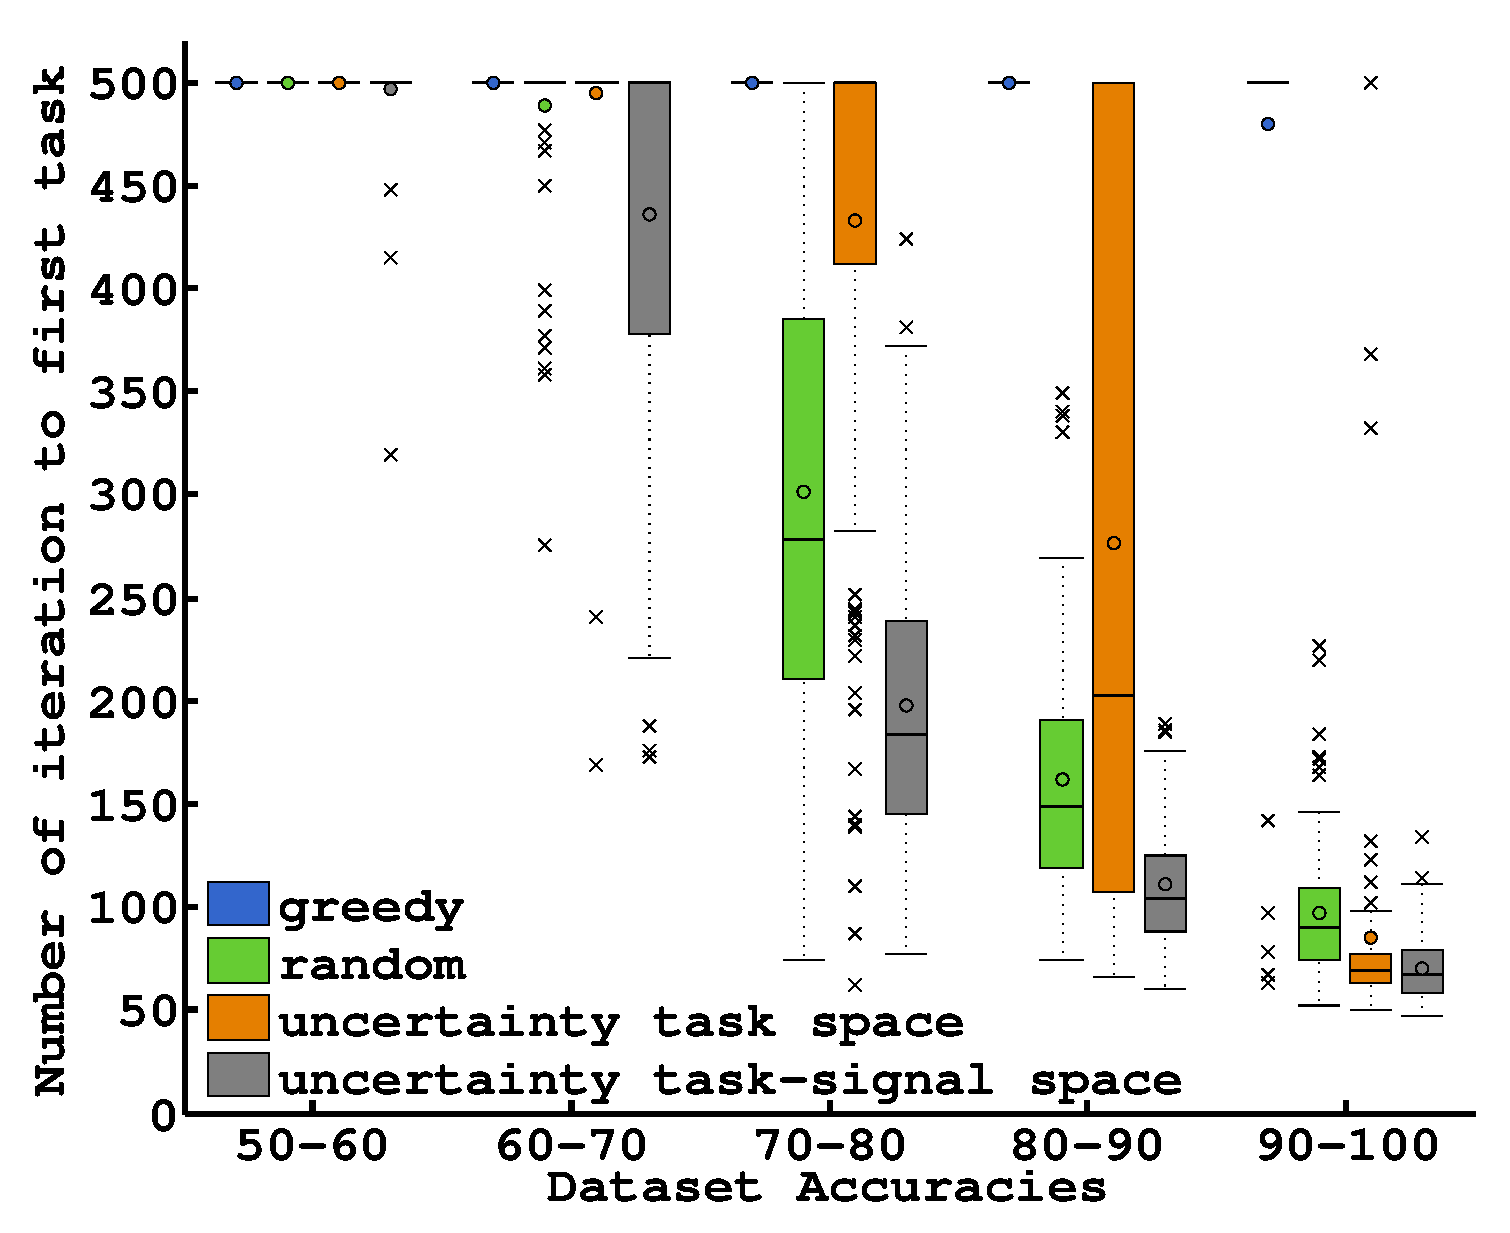
\includegraphics[width=\columnwidth]{img/plots_aaai/plot_artificial_planning.eps}
      \caption{Number of steps to complete first task, comparison of different exploration methods with 30 dimensional artificial data. When learning from scratch, planning upon uncertainty in both task and signal space performs better than relying only on task uncertainty. Greedy action selection rarely disambiguates between hypothesis.}
    \label{fig:planning}
\end{figure}

As depicted in Figure~\ref{fig:planningExplained}, the system needs to collect two types of information, some about the true underlying model (Fig.~\ref{fig:planningExplained}b) and some to differentiate between hypotheses (Fig.~\ref{fig:planningExplained}a). The properties of the grid world make the random strategy quite efficient at collecting those two types of information. The differences between planning methods should be more evident when navigating a complex maze since our method allows to plan in order to collect the type of information we need. Studying how different world properties affect the learning efficiency is part of our future work. Also, we note that all planning methods were switched to pure exploitation (greedy) once the confidence level was reached. Therefore the performance in Figure~\ref{fig:planning} compares the ability of the different methods to discriminate between different task hypotheses, not their ability to solve the task itself.

\paragraph{Dimensionality}

Figure~\ref{fig:firstArtificial} compares the number of steps (with maximum values of 500 steps) needed to identify the first task when learning from scratch with different dimensionality of datasets. The convergence speed is only slightly affected by the features dimensionality. On the other hand, the dataset quality (measured in terms of it associated ten-fold accuracy) is the main cause of performances decay. Furthermore, for those datasets with accuracies between $50\%$ and $60\%$, the system is not able to identify a task with confidence after 500 steps.

\begin{figure}[!ht]
  \centering
      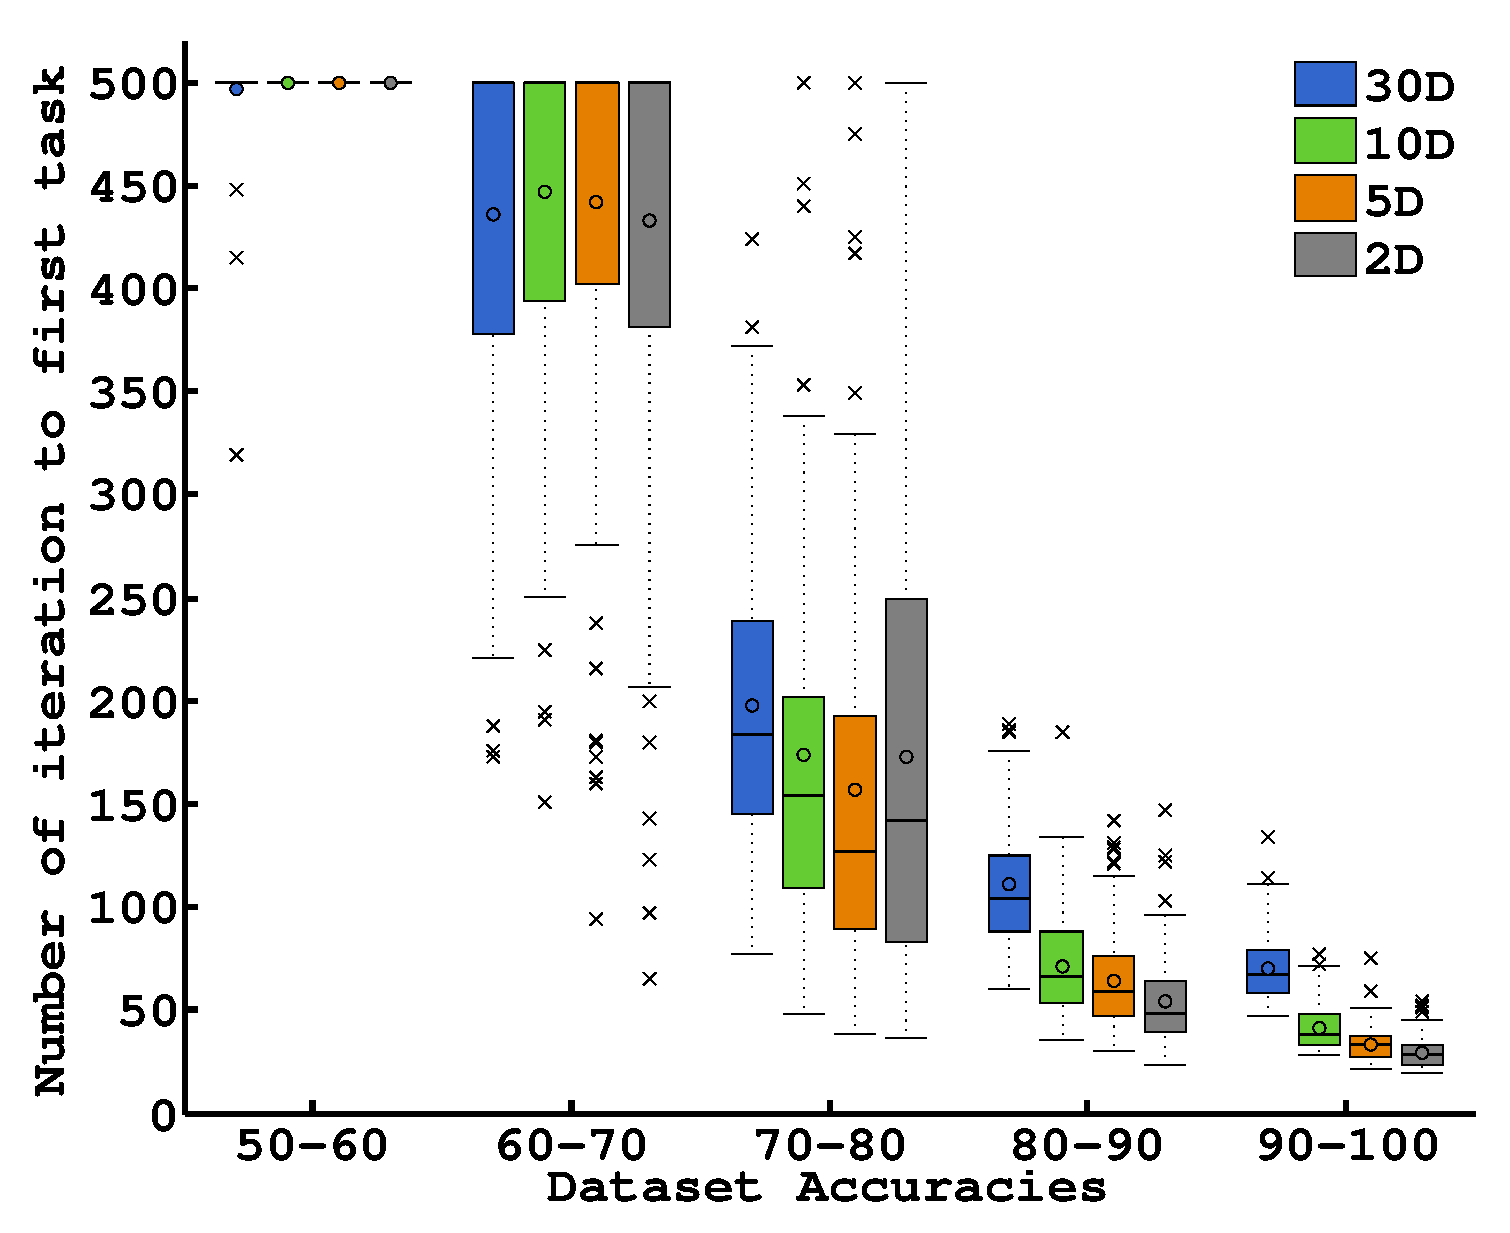
\includegraphics[width=\columnwidth]{img/plots_aaai/plot_artificial_firstconf.eps}
      \caption{Number of steps to complete first task using artificial data. Under 60 percent accuracy, the confidence threshold cannot be reached in 500 steps. The dataset qualities, more than their dimensionality, impact the learning time.}
      \label{fig:firstArtificial}
\end{figure} 

Once one task is completed, a new one is selected randomly. Figure~\ref{fig:nCorrectArtificial} compares the number of tasks that can be achieved in 500 steps. As expected, the lower the quality of the data, the less number of task can be completed. With dataset accuracies higher than $90\%$ we can achieve more than 30 tasks on average.

\begin{figure}[!ht]
    \centering
    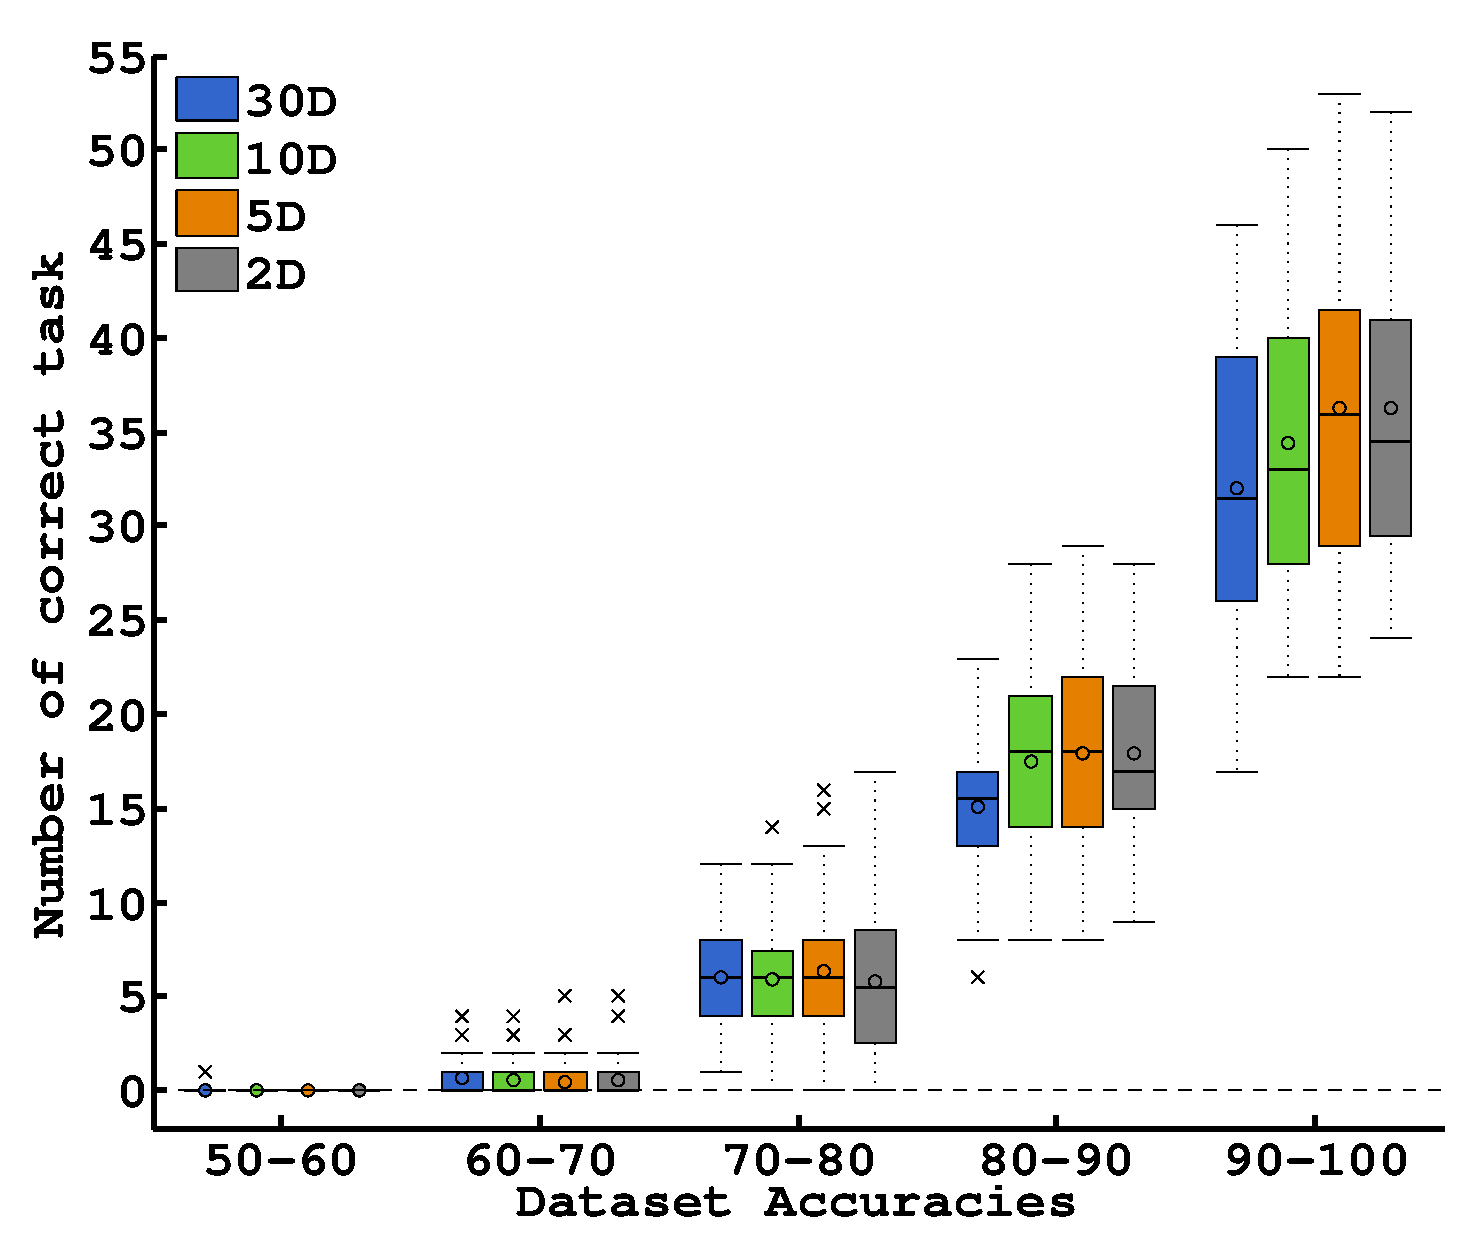
\includegraphics[width=\columnwidth]{img/plots_aaai/plot_artificial_nCorrect.eps}
    \caption{Number of tasks correctly achieved in 500 steps, artificial data. Quality of dataset impacts the number of task identified in 500 steps as more evidence should be collected to reach the confidence threshold.}
    \label{fig:nCorrectArtificial}
\end{figure} 

An important aspect of the proposed learning approach was that the first task learned was always the correct one. We reported only 9 erroneous estimations across all simulated experiments (5 in the 70-80 group and 4 in the 80-90 group).

\subsection{EEG datasets and comparison with calibration method}

\paragraph{Example}
Figure~\ref{fig:sequence} shows one particular run of 500 steps comparing our self-calibration method with a calibration procedure of 400 steps. The two independent runs use as real EEG dataset with $80\%$ ten-fold classification accuracy. As our algorithm is operational from the first step, it can estimate the real task when sufficient evidence has been collected. On the other hand, a calibration approach collects signal-label pairs for a fixed number of steps and use the resulting classifier without updating it. This provokes that, during the calibration phase, no tasks can be learned, substantially delaying the user's online operation.

\begin{figure}[!ht]
\centering
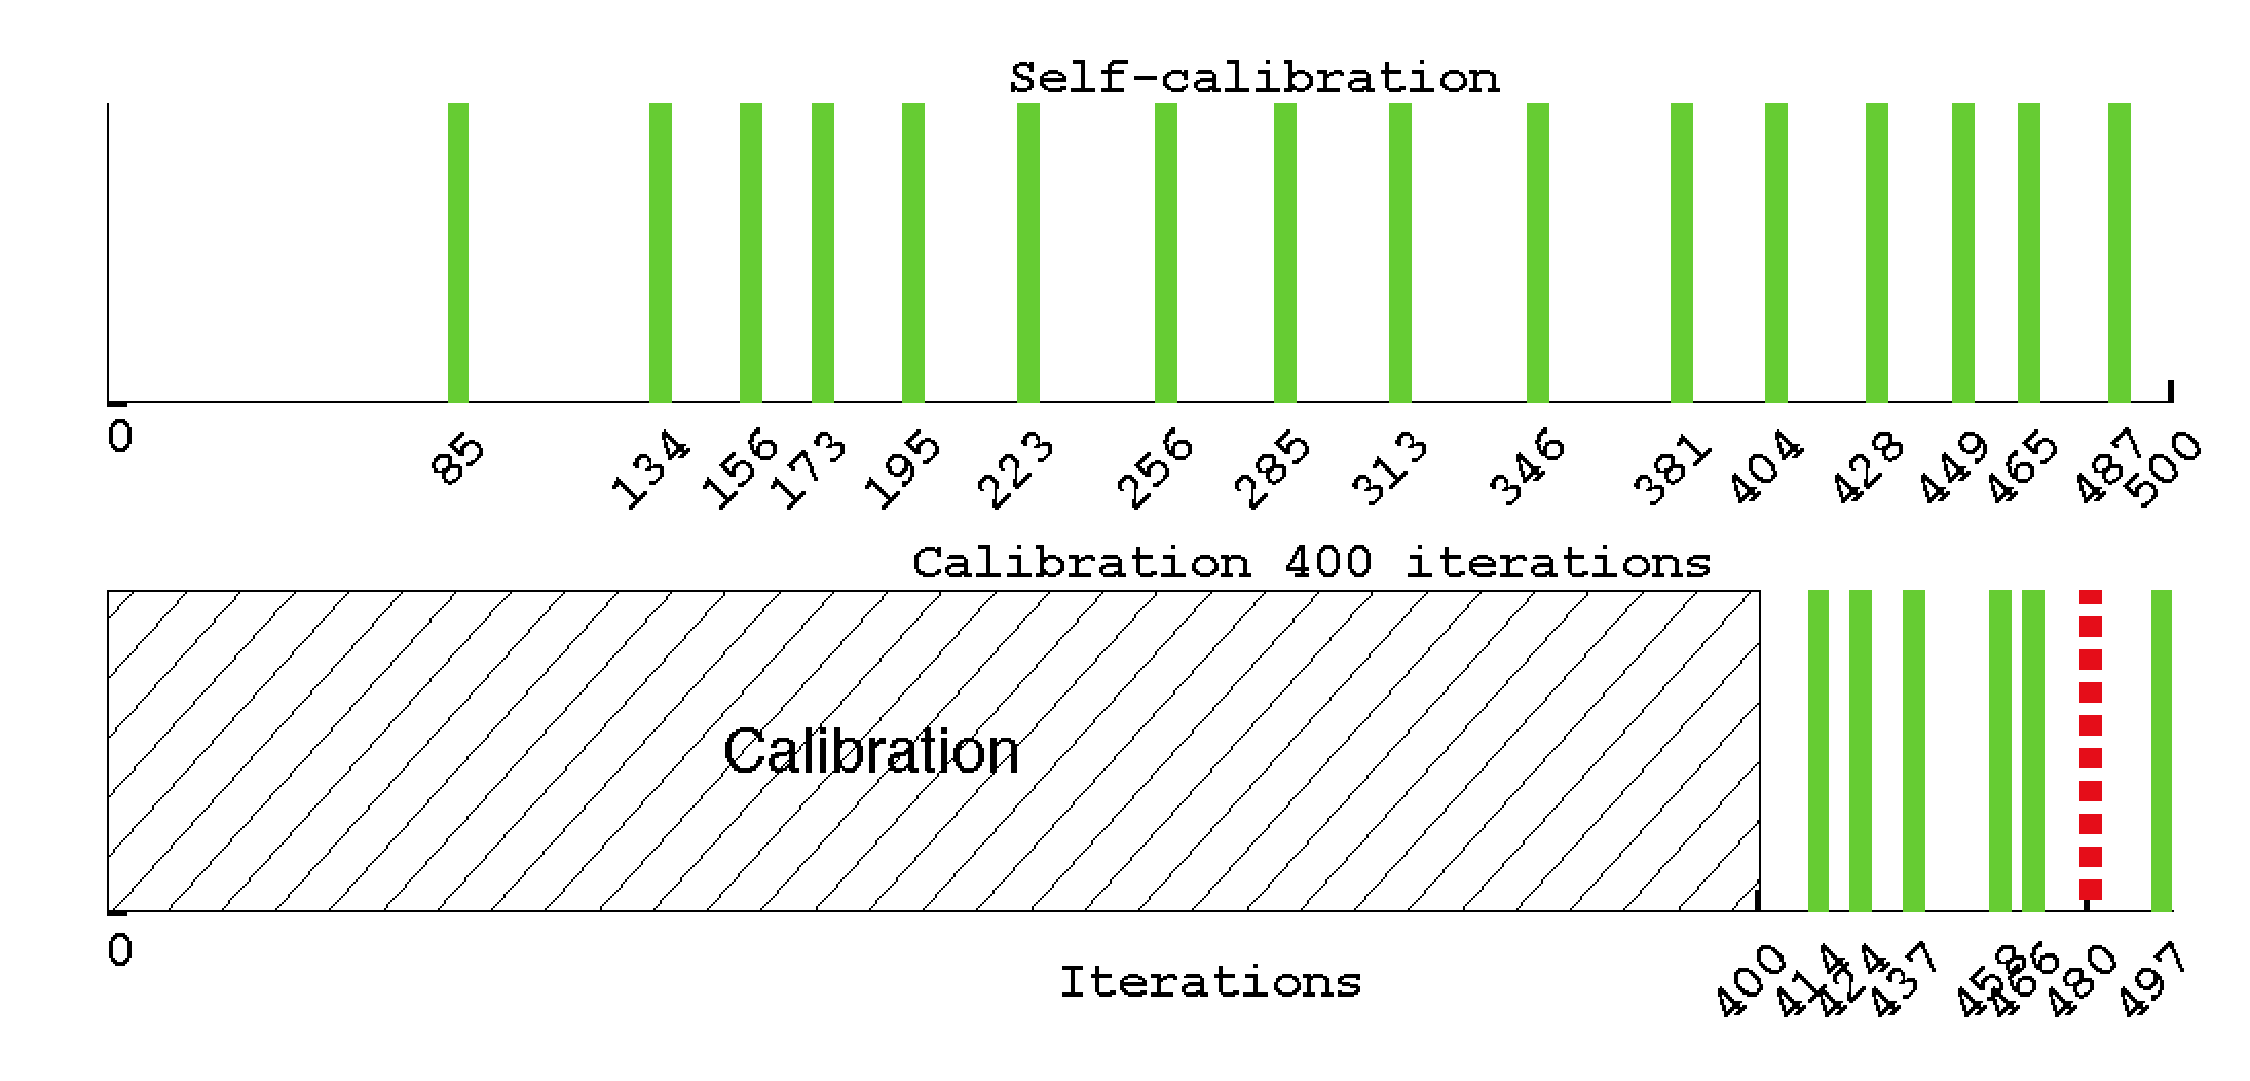
\includegraphics[width=\columnwidth]{img/plots_aaai/plot_the_aaai_sequence.eps}
\caption{Time-line of one run from EEG dataset of $80$ percent ten-fold classification accuracy, self-calibration (top) versus 400 steps calibration (bottom). Green (filled) and red (dashed) bars represents respectively correct and incorrect task achievement. The proposed self-calibration method allow to reach a first task faster than would take a calibration procedure.}
\label{fig:sequence}
\end{figure} 



Figure~\ref{fig:sequence_evolution} shows the evolution of classification rate between our self-calibration method with a calibration procedure of 400 steps. As our method assigns different labels to each new teaching signal, the resulting classifiers have different performances, which help identifying the correct task. Once a task is identified (e.g.\ step 85 and 134), the corresponding labels are taken as ground truth, and all classifiers will have the same accuracies. As the agent starts exploring again to estimate the new tasks, all the classifiers except the true one will start to have worse accuracies again.

\begin{figure}[!ht]
\centering
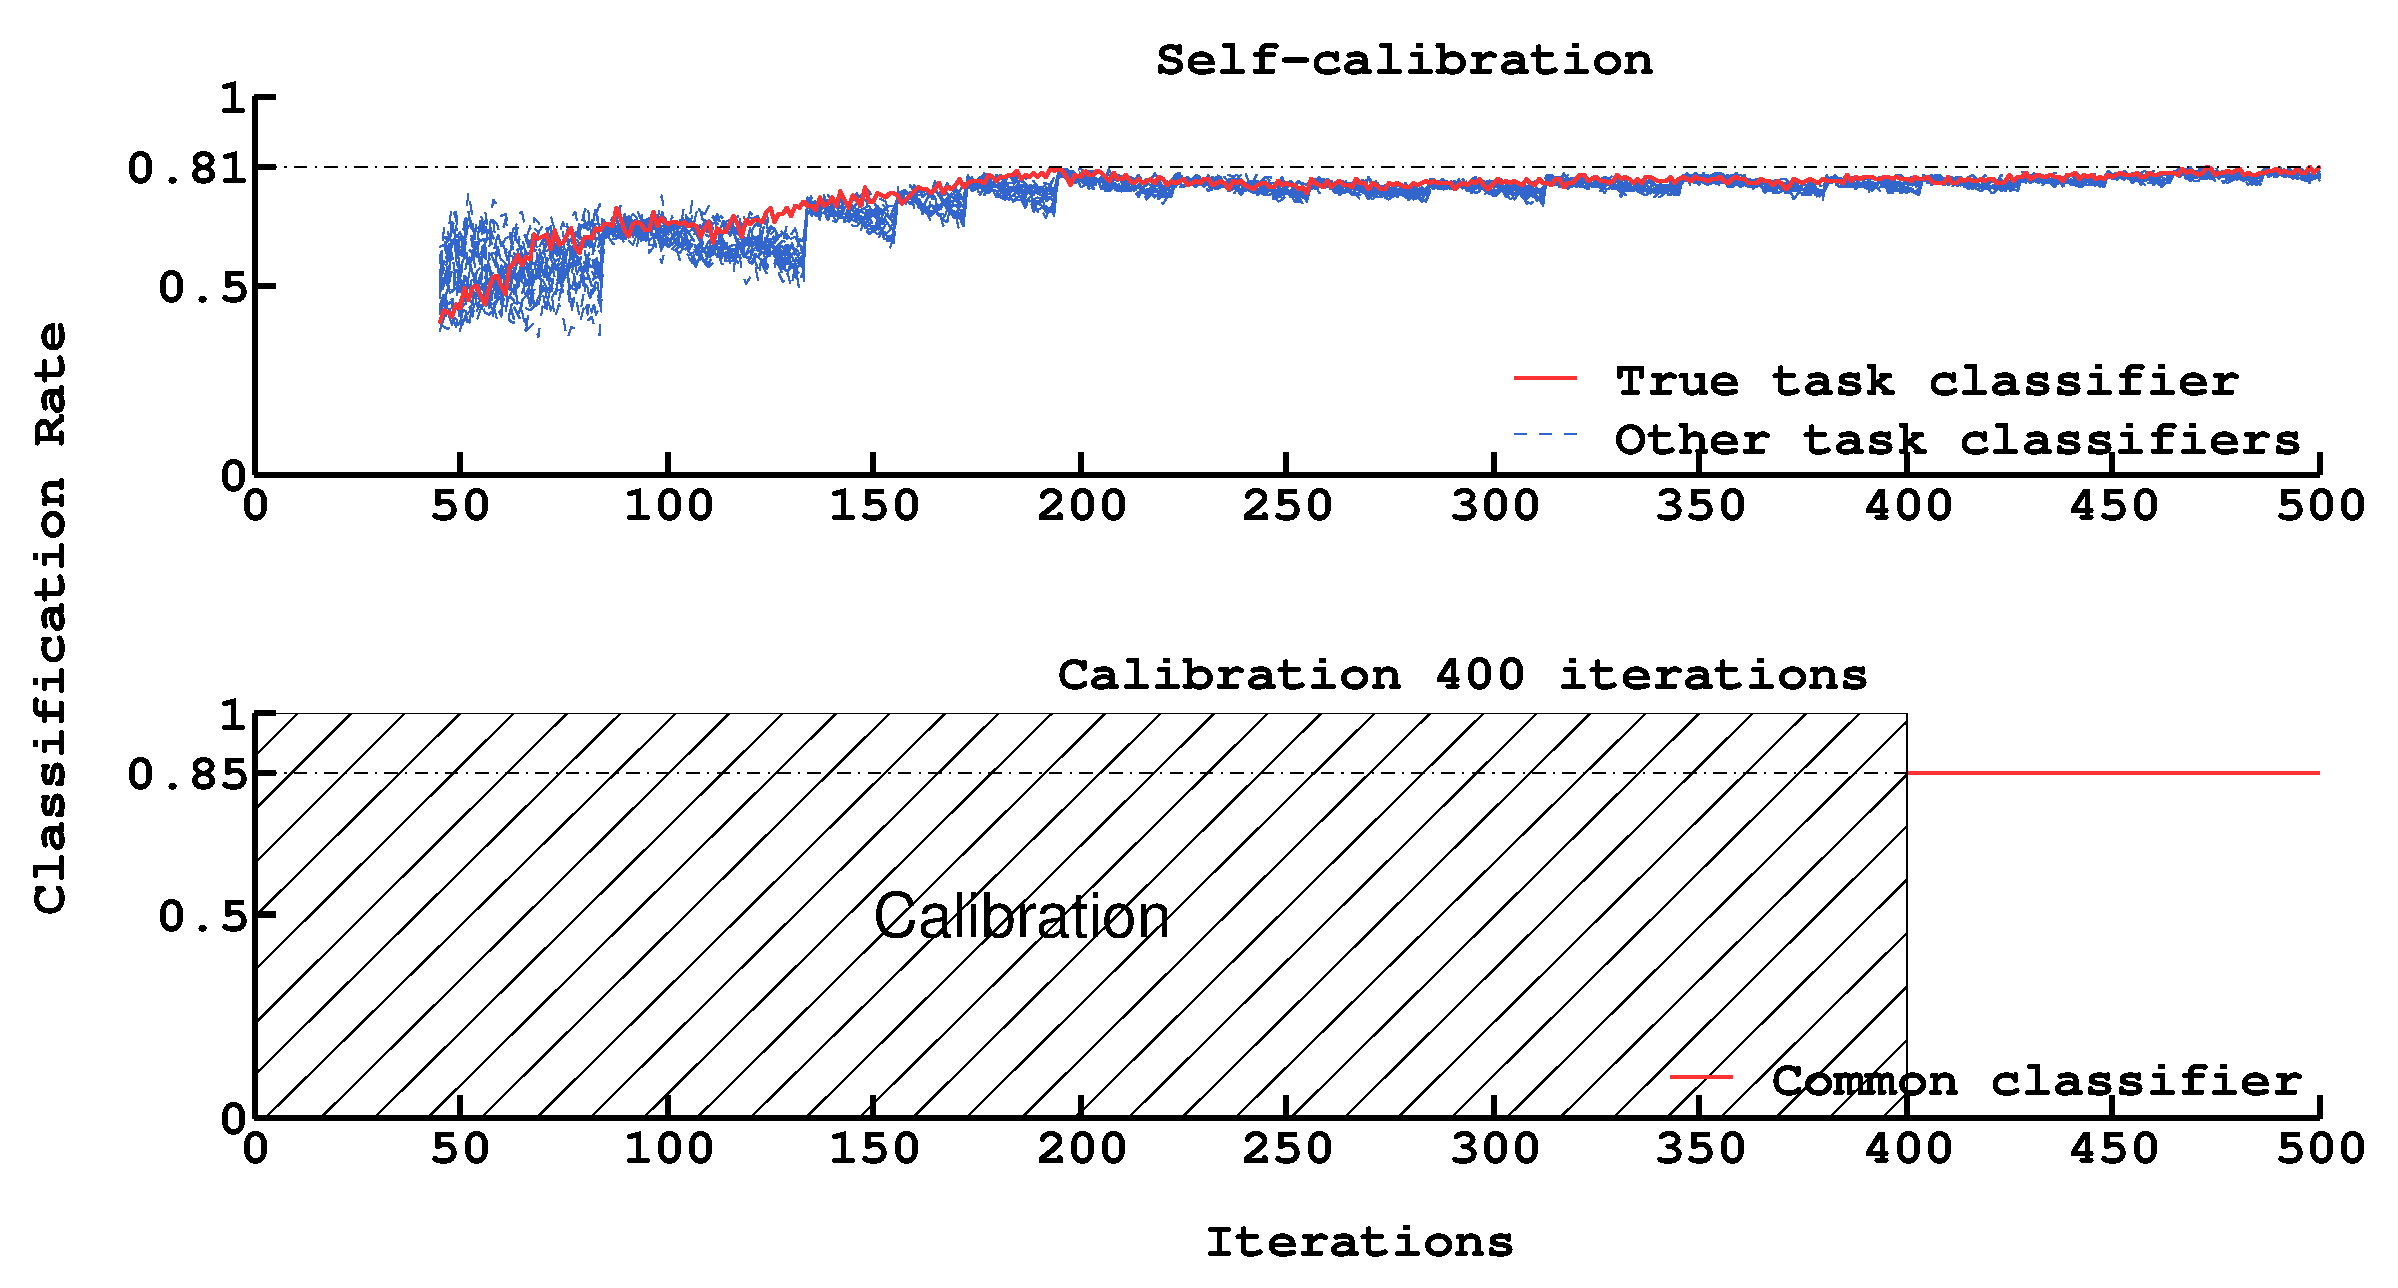
\includegraphics[width=\columnwidth]{img/plots_aaai/plot_evo_classification_rate.eps}
\caption{Evolution of classification rate of one run from EEG data, self-calibration (top) versus 400 steps calibration (bottom). On top, the red line represents the classifier corresponding to the successive tasks taught by the user, the dashed blue lines represent all others tasks. Our method updates classifiers every steps.}
\label{fig:sequence_evolution}
\end{figure} 

\paragraph{Time to first task}

Figure~\ref{fig:firstEEG} shows the results per group of dataset. Our algorithm allows to complete the first task without errors and in a fair amount of iteration.  For our method, the learning time is strongly correlated with the dataset quality. However calibration methods, which do not update their classifier once calibrated, identify more tasks incorrectly.

\begin{figure}[!ht]
\centering
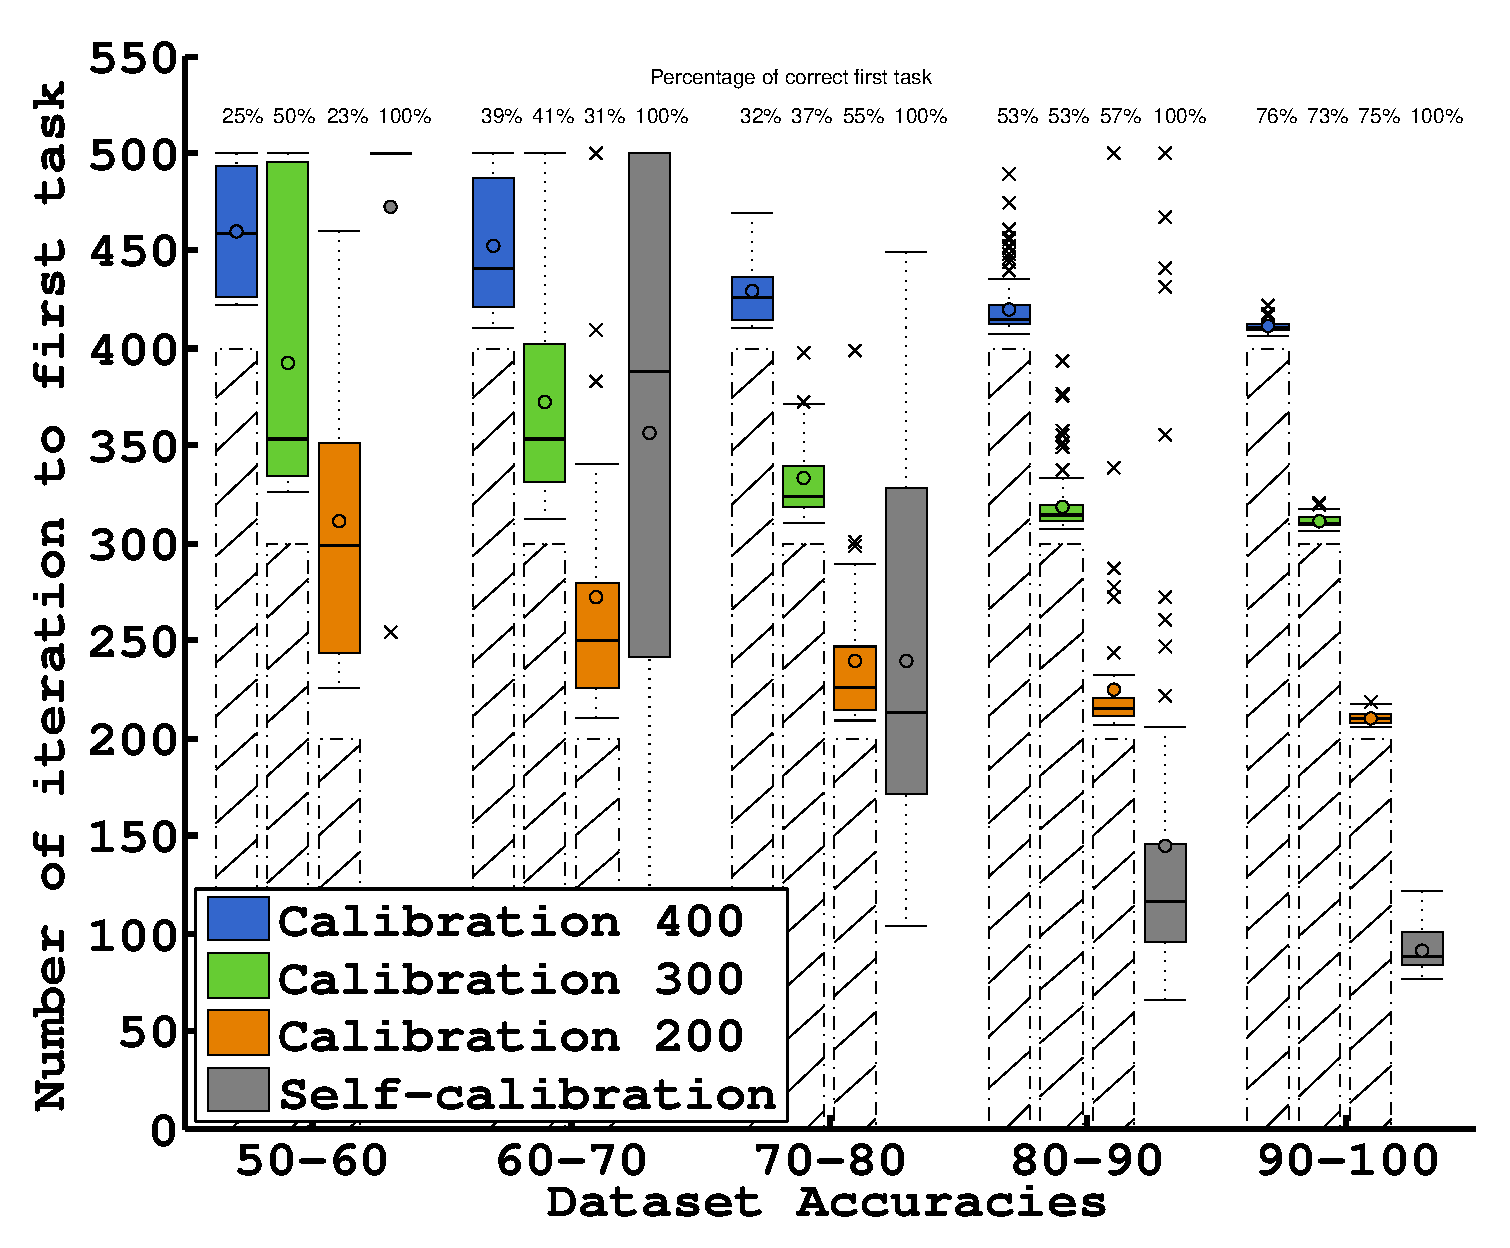
\includegraphics[width=\columnwidth]{img/plots_aaai/plot_EEG_calib_firstconf.eps}
\caption{Number of steps to complete first task with EEG data. The method scale well to EEG data. Contrary to the standard calibration approaches, we do not make mistakes with low quality datasets.}
\label{fig:firstEEG}
\end{figure} 

%We can identify two main differences between our method and the usual calibration procedure for this kind of BCI experiments:
%\begin{enumerate}
%\item \textbf{Positive/Negative percent ratio of training examples}. Following the literature \cite{chavarriaga2010learning, iturrate2013task} we used a 80/20 percent ratio. Table \ref{tab:correctLabelRatio} shows the positive/negative ratio obtained following our planning method. The ratio we obtain is more balanced, resulting in classifiers with better properties. However a 50/50 percent ratio may lead to practical problems during online real world experiments and should be studied in more details, see open questions in section \ref{sec:conclusion}.
%\item \textbf{Online update of multiple classifiers.} Our method integrates new data at every step whose label can differ between task hypothesis. For incorrect task hypothesis, the associated label can be incorrect and decrease the performance of the associated classifier, see figure \ref{fig:planningExplained}c. This dynamic can be observed in figure \ref{fig:sequence_evolution} where classifiers associated to incorrect tasks (in blue) have lower estimated accuracies than the correct one (in red). As a result our algorithm makes different predictions and updates for each hypothesis.
%\end{enumerate}

%\begin{table}
%\begin{tabular}{c c c}
%Dataset Accuracies & Self-calibration & Calibration \\ \hline
%50-60 & 0.48 (0.02) & 0.8 (0) \\
%60-70 & 0.50 (0.03) & 0.8 (0) \\
%70-80 & 0.53 (0.03) & 0.8 (0) \\
%80-90 & 0.57 (0.03) & 0.8 (0) \\
%90-100 & 0.59 (0.01) & 0.8 (0) \\
%\end{tabular}
%\caption{Mean ratio of positive examples in training dataset (standard deviation shown in parenthesis). Calibration procedure for ErP EEG signal usual account for a 80 percent ratio of positive examples. However when following our method we collect as many positive than negative examples, see discussion in section \ref{sec:conclusion}.}
%\label{tab:correctLabelRatio}
%\end{table}

%\begin{figure}[!ht]
%\centering
%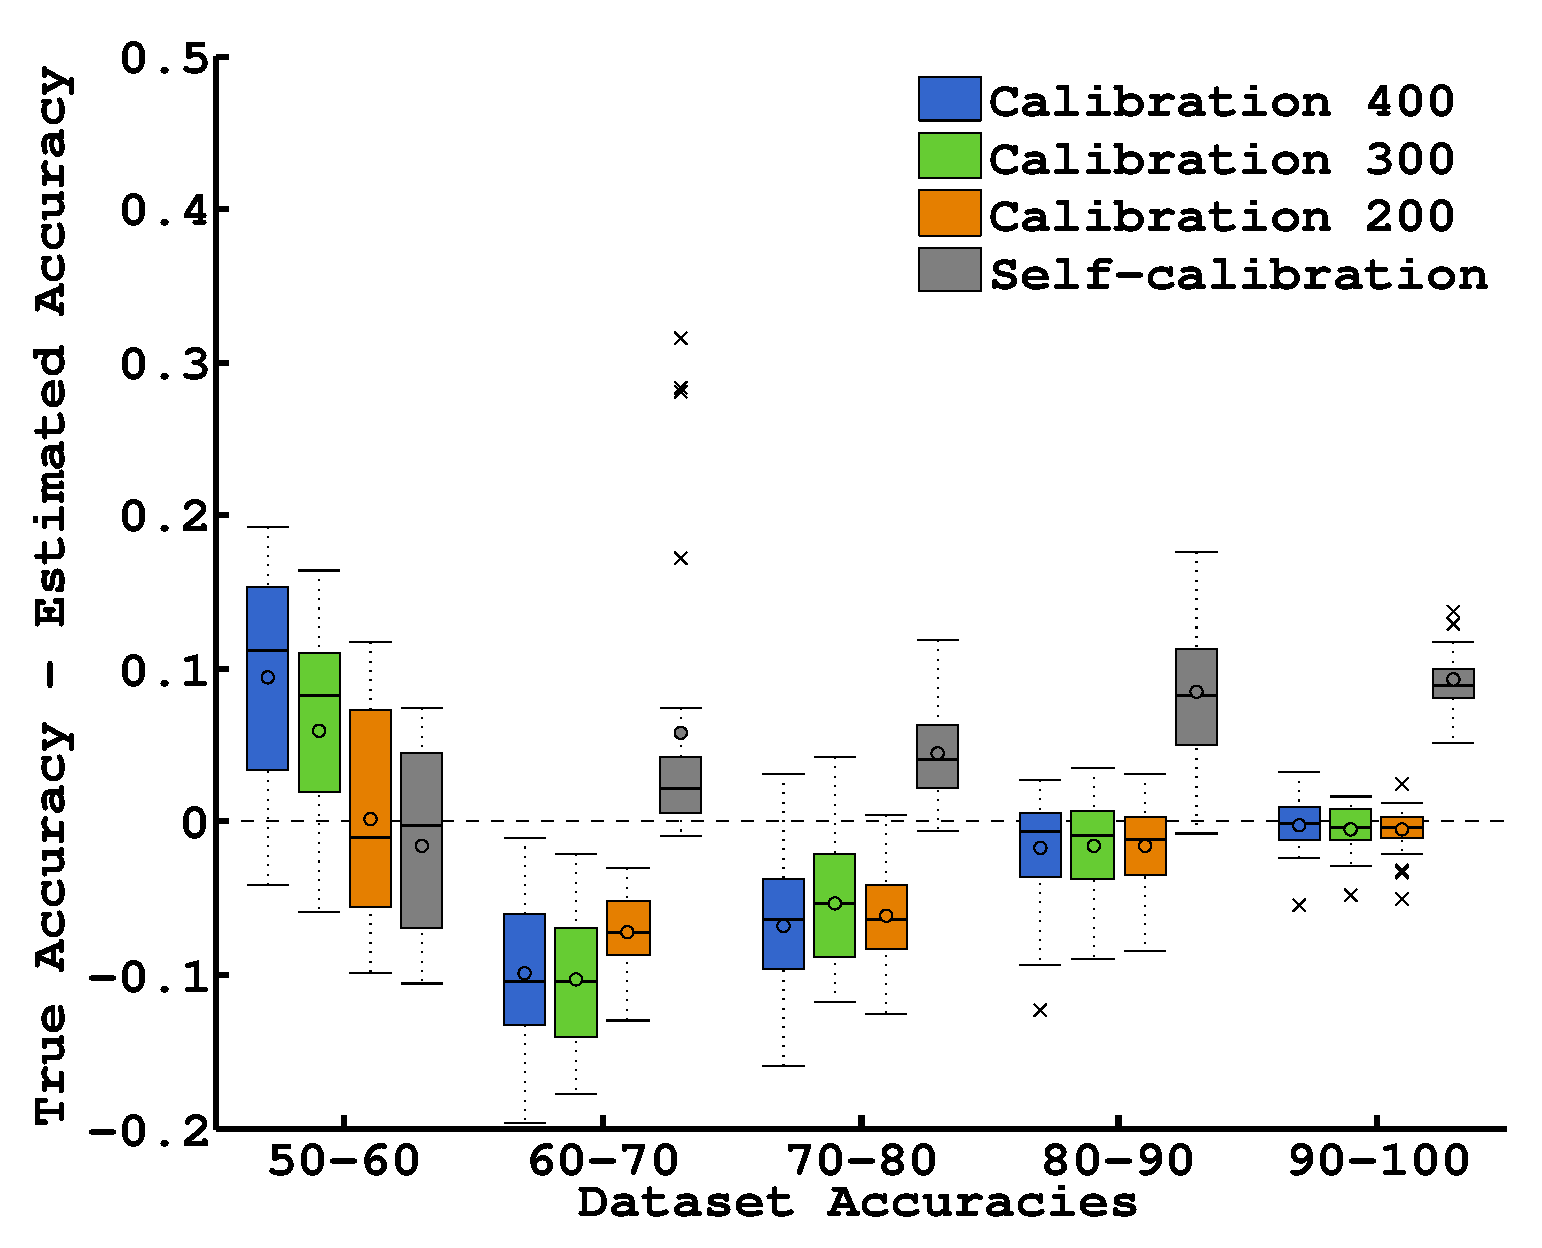
\includegraphics[width=\columnwidth]{img/plots_aaai/plot_explaination_for_calib_failure.eps}
%\caption{Difference between true accuracy and estimated accuracy. True accuracy is the performance of the classifier on the unused data. Estimated accuracy is the 10 fold cross validation performance of the classifier on collected data. A negative(positive) value indicates the classifier is over(under)-estimating its performance. Calibration methods tend to produce over-confident classifiers, certainly due to the biased positive to negative training example ratio, see table \ref{tab:correctLabelRatio}.}
%\label{fig:calibFail}
%\end{figure}

\paragraph{Cumulative performances}

Figure~\ref{fig:nCorrectEEG} compares the number of tasks that can be achieved in 500 steps. With 90\% and more dataset quality we can achieve about 20 tasks on average. The results are consistent with artificial dataset analysis.

\begin{figure}[!ht]
\centering
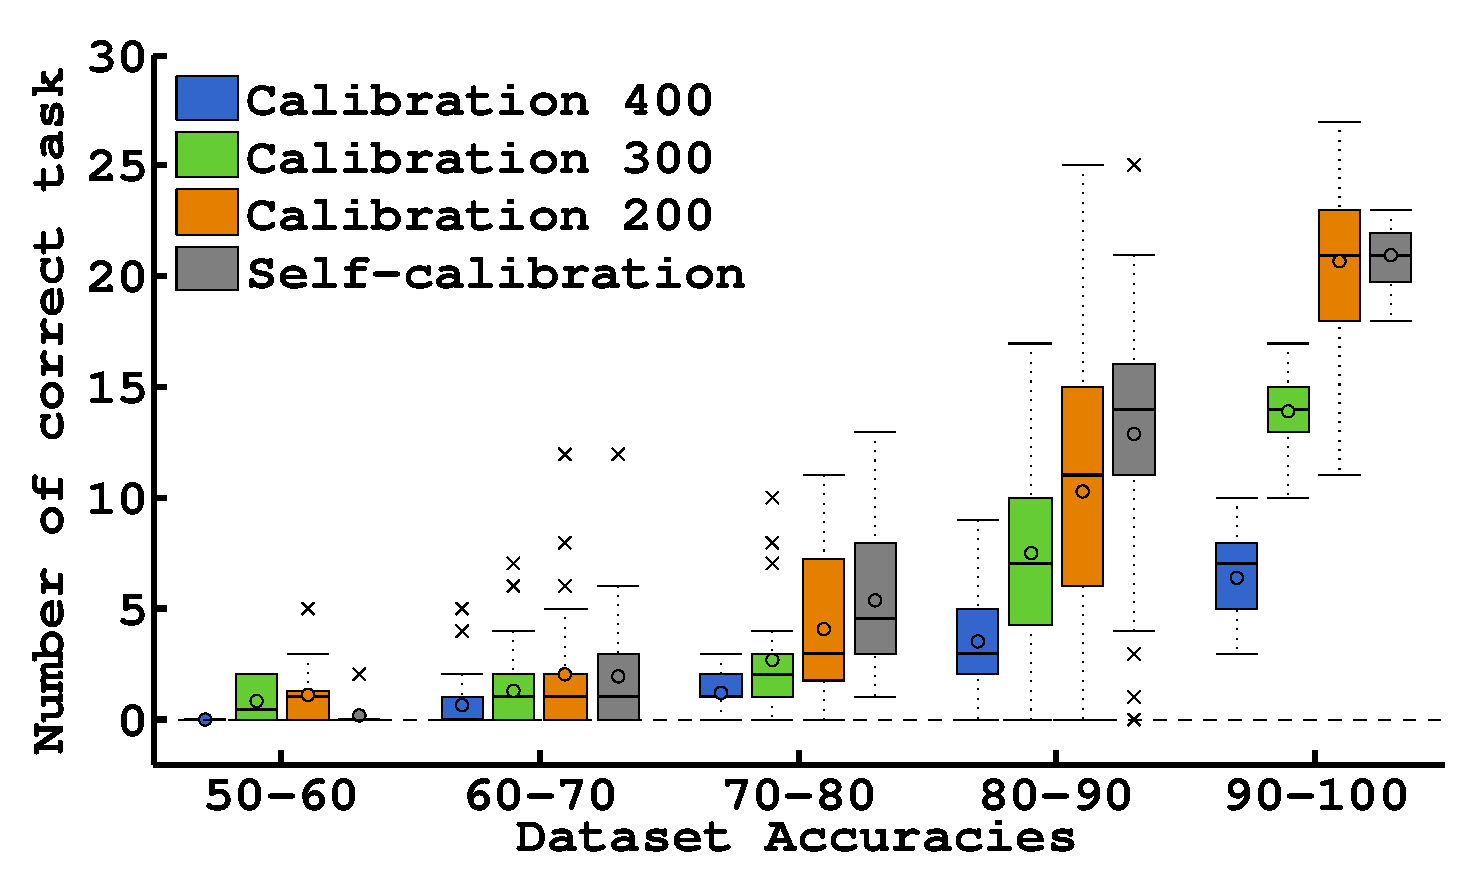
\includegraphics[width=\columnwidth]{img/plots_aaai/plot_EEG_calib_nCorrect.eps}
\caption{Number of task correctly achieved in 500 steps with EEG data. Calibration methods can not complete a significant number of task as most of the time is spent on calibration.}
\label{fig:nCorrectEEG}
\end{figure} 

The calibration methods can not complete many task as a significant amount of iteration was used for calibrating the system. A calibration of 200 steps makes as many good estimation than our method, but it also makes many wrong estimation, see Figure~\ref{fig:nWrongEEG}. For calibration methods, the less time spent on calibration, the poorer the classifier which implies more mistakes.

\begin{figure}[!ht]
\centering
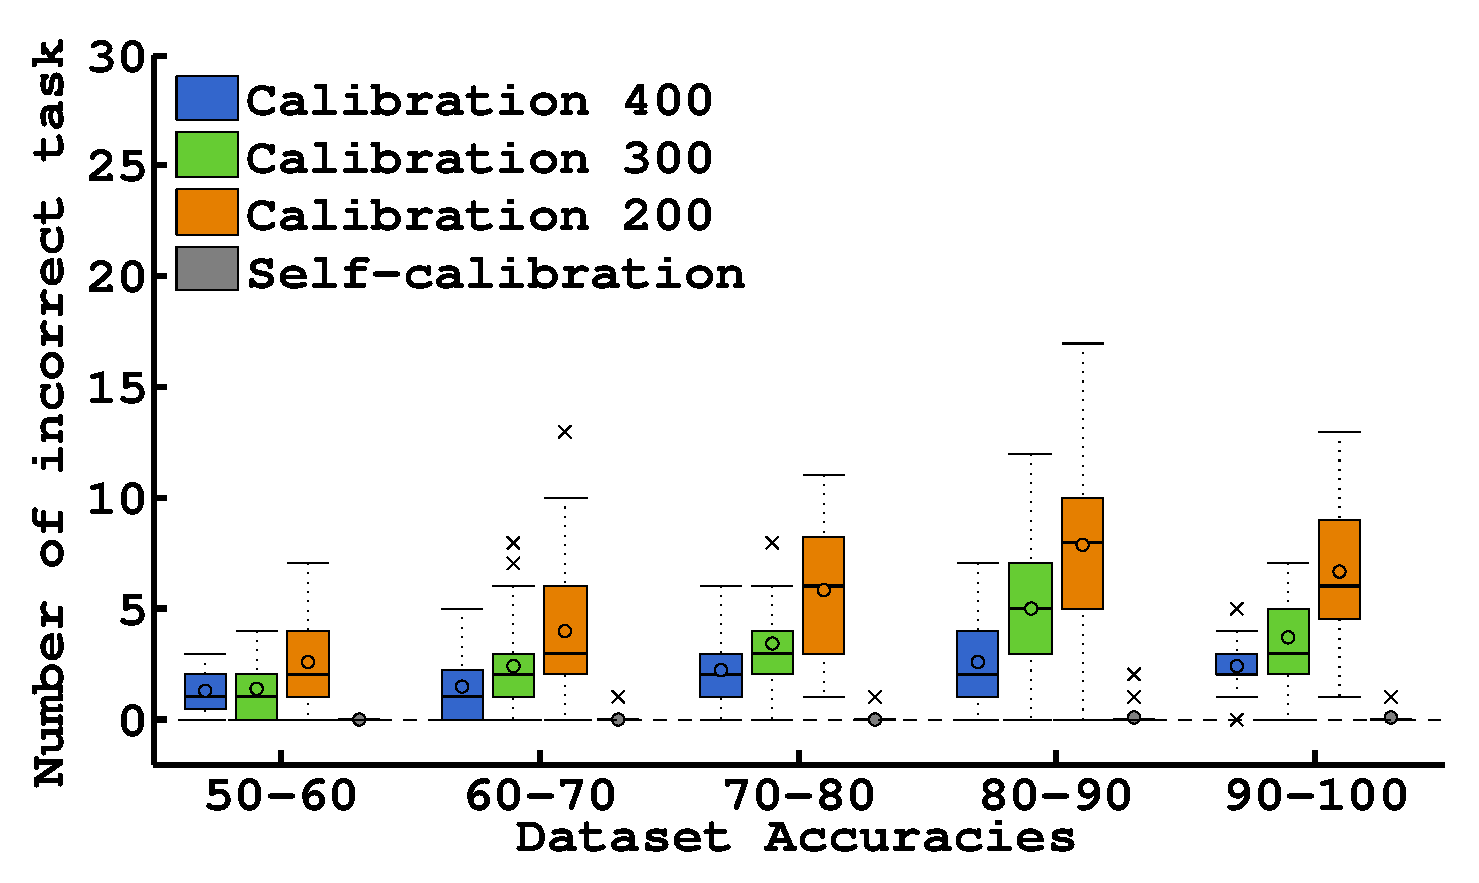
\includegraphics[width=\columnwidth]{img/plots_aaai/plot_EEG_calib_nWrong.eps}
\caption{Number of task incorrectly achieved in 500 steps with EEG data. Calibration methods, which do not update their models once calibrated, make more errors.}
\label{fig:nWrongEEG}
\end{figure}

%\paragraph{Last 100 iterations performances}
%
%Figure~\ref{fig:nCorrectEEG_last100} compares the number of task that can be achieved during the last 100 steps with EEG data. With 80-90\% dataset quality, all methods achieve an average success rate of one task every 20 steps. However calibration methods, which do not update their models once calibrated, make more mistakes (see figure \ref{fig:nWrongEEG_last100}).
%
%\begin{figure}[!ht]
%\centering
%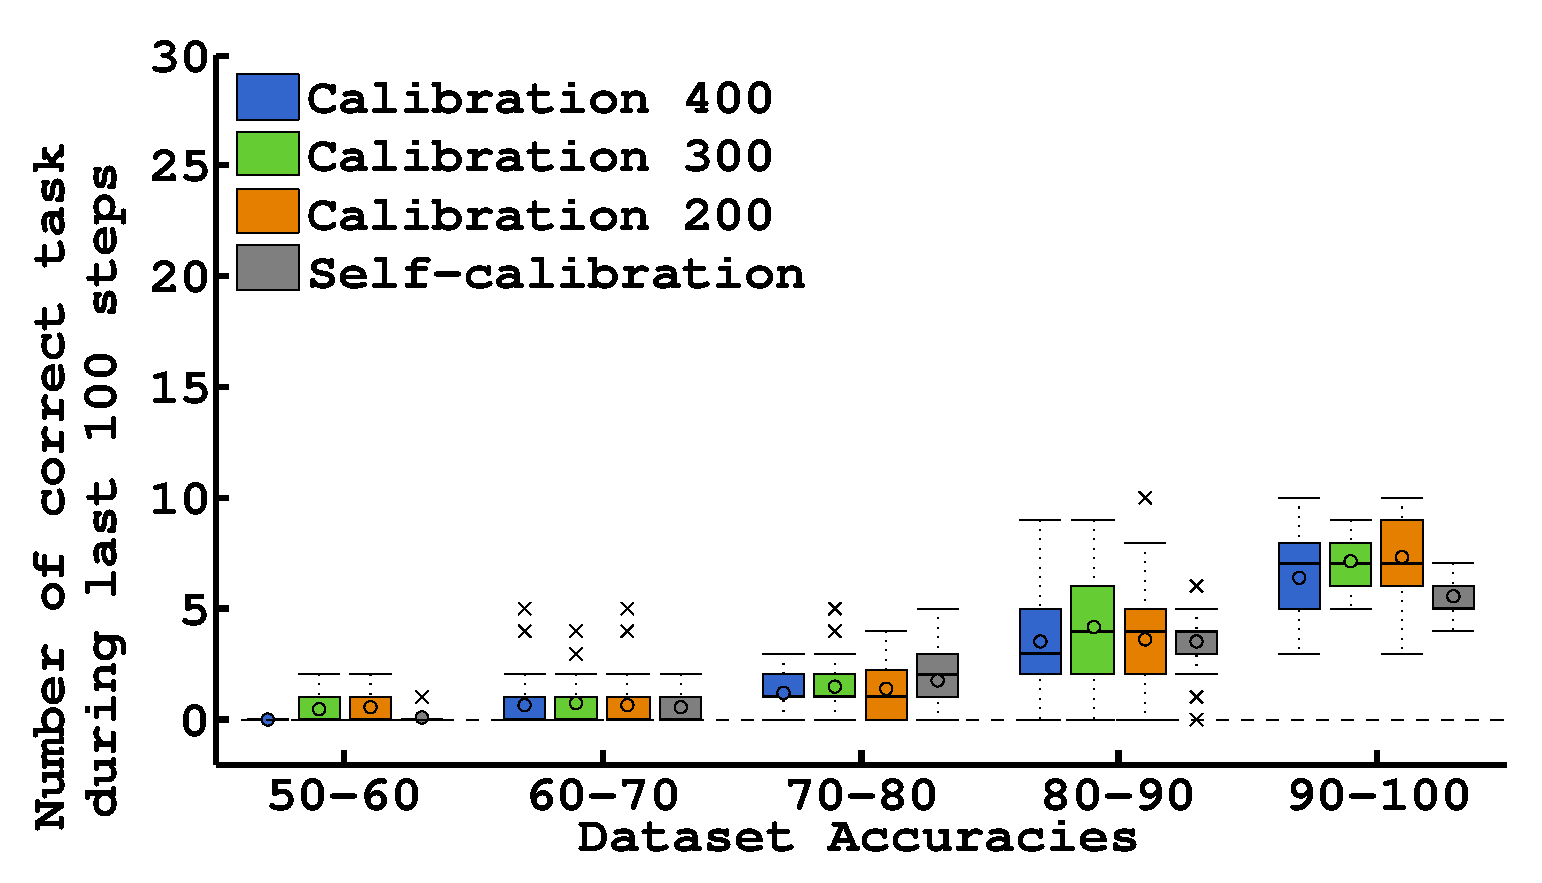
\includegraphics[width=\columnwidth]{img/plots_aaai/plot_EEG_calib_nCorrect_last100.eps}
%\caption{Number of task correctly achieved during the last 100 steps with EEG data. All methods have equivalent successful reaching rate.}
%\label{fig:nCorrectEEG_last100}
%\end{figure} 
%
%\begin{figure}[!ht]
%\centering
%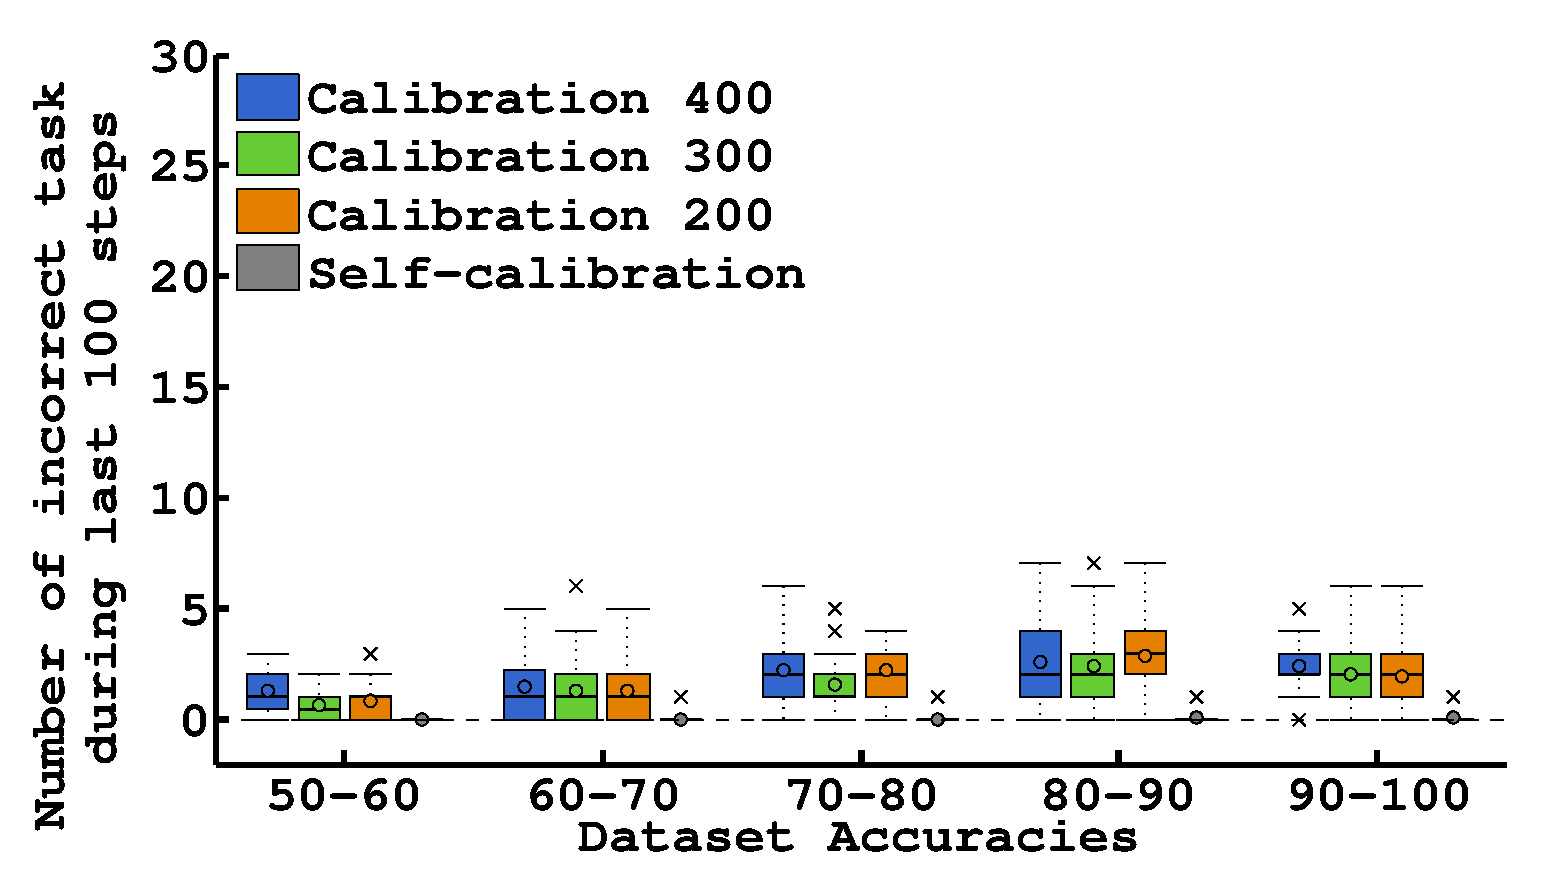
\includegraphics[width=\columnwidth]{img/plots_aaai/plot_EEG_calib_nWrong_last100.eps}
%\caption{Number of task incorrectly achieved during the last 100 steps with EEG data. Calibration methods, which do not update their models once calibrated, make more errors.}
%\label{fig:nWrongEEG_last100}
%\end{figure} 

 % shows the number of tasks identified with respect to the accuracy of the dataset, and the number of tasks incorrectly identified. Notice how the number of identified task is correlated to the quality of the dataset. Importantly, we were able to identify 15 to 20 tasks in 500 steps on good quality dataset without the need for a calibration procedure.


% \begin{figure*}[t]
% \centering
% \begin{minipage}[t]{.65\columnwidth}
% 	\centering
%    		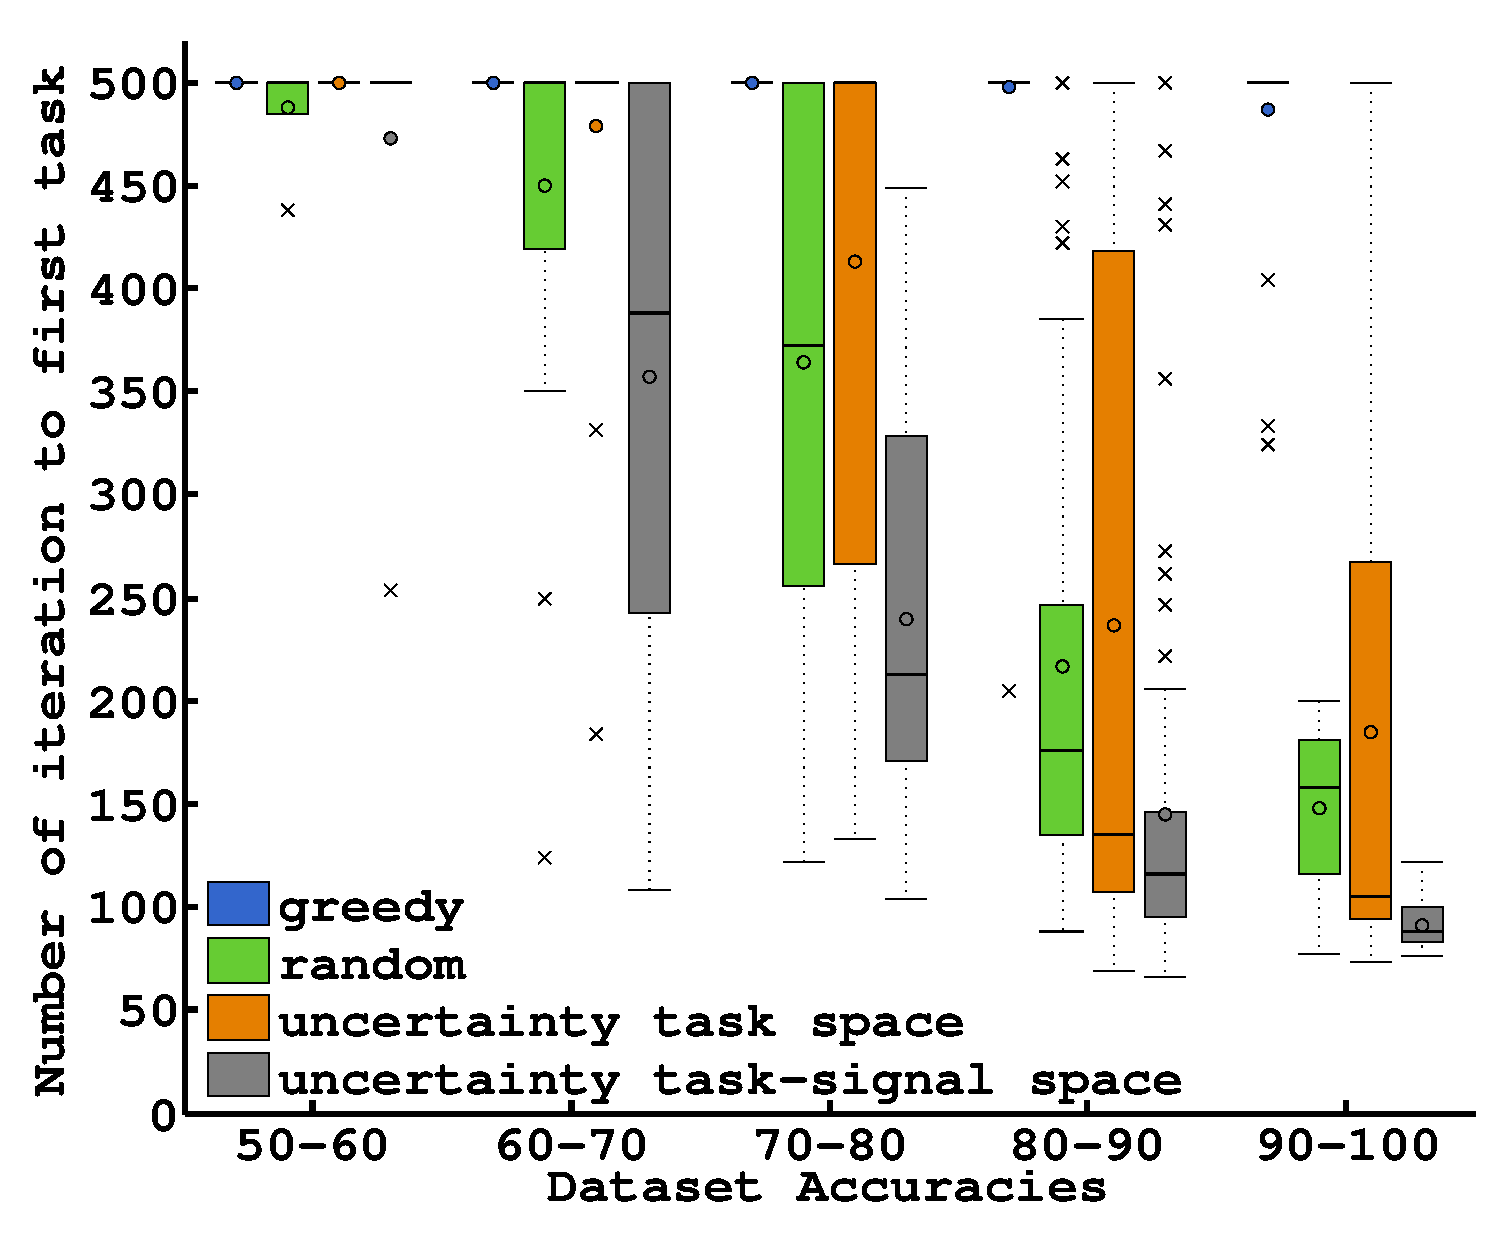
\includegraphics[width=\columnwidth]{img/plots_aaai/plot_EEG_planning.eps}
%    		\caption{\todo{this is the plot for EEG data, xp are running for artificial data}}
% 		\label{fig:planning}
% \end{minipage}
% \begin{minipage}[t]{.65\columnwidth}
% 	\centering
%    		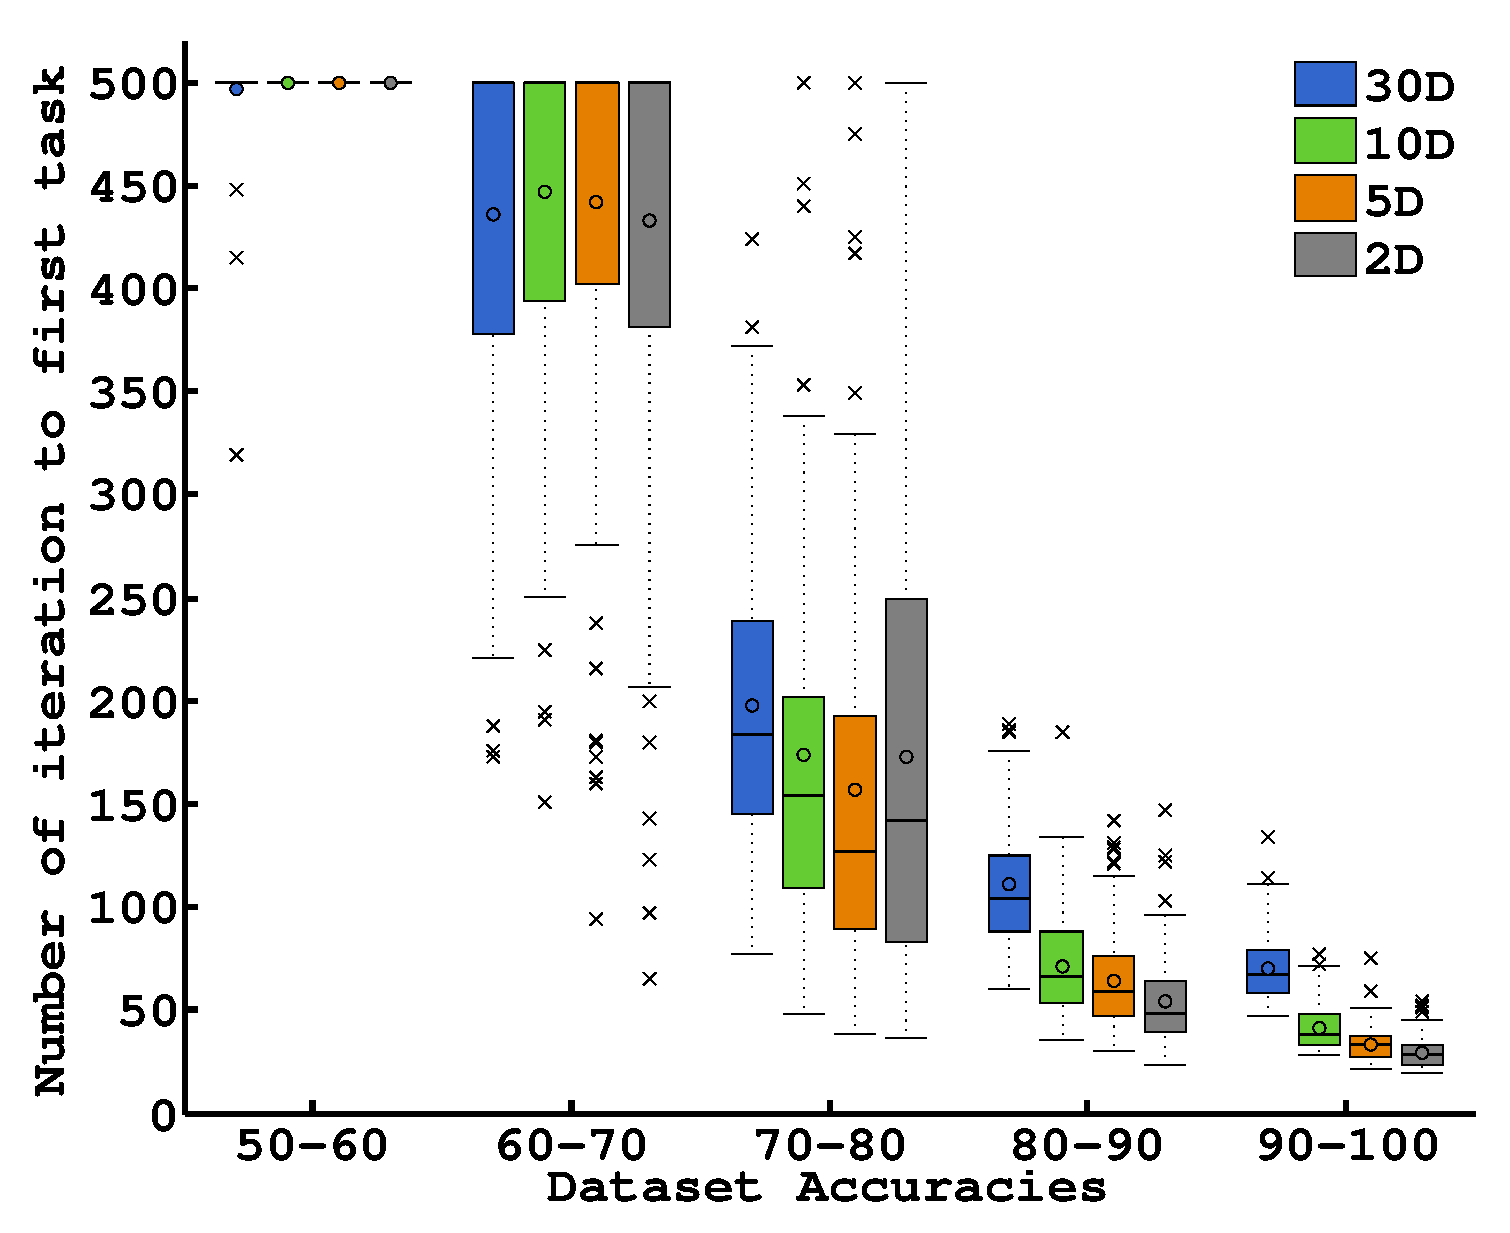
\includegraphics[width=\columnwidth]{img/plots_aaai/plot_artificial_firstconf.eps}
%    		\caption{Under 70 percent accuracy, the confidence threshold cannot be reached in 500 steps. The dataset qualities, more than their dimensionality, impact the learning time.}
%    		\label{fig:firstArtificial}
% \end{minipage}	
% \begin{minipage}[t]{.65\columnwidth}
% 	\centering
%    			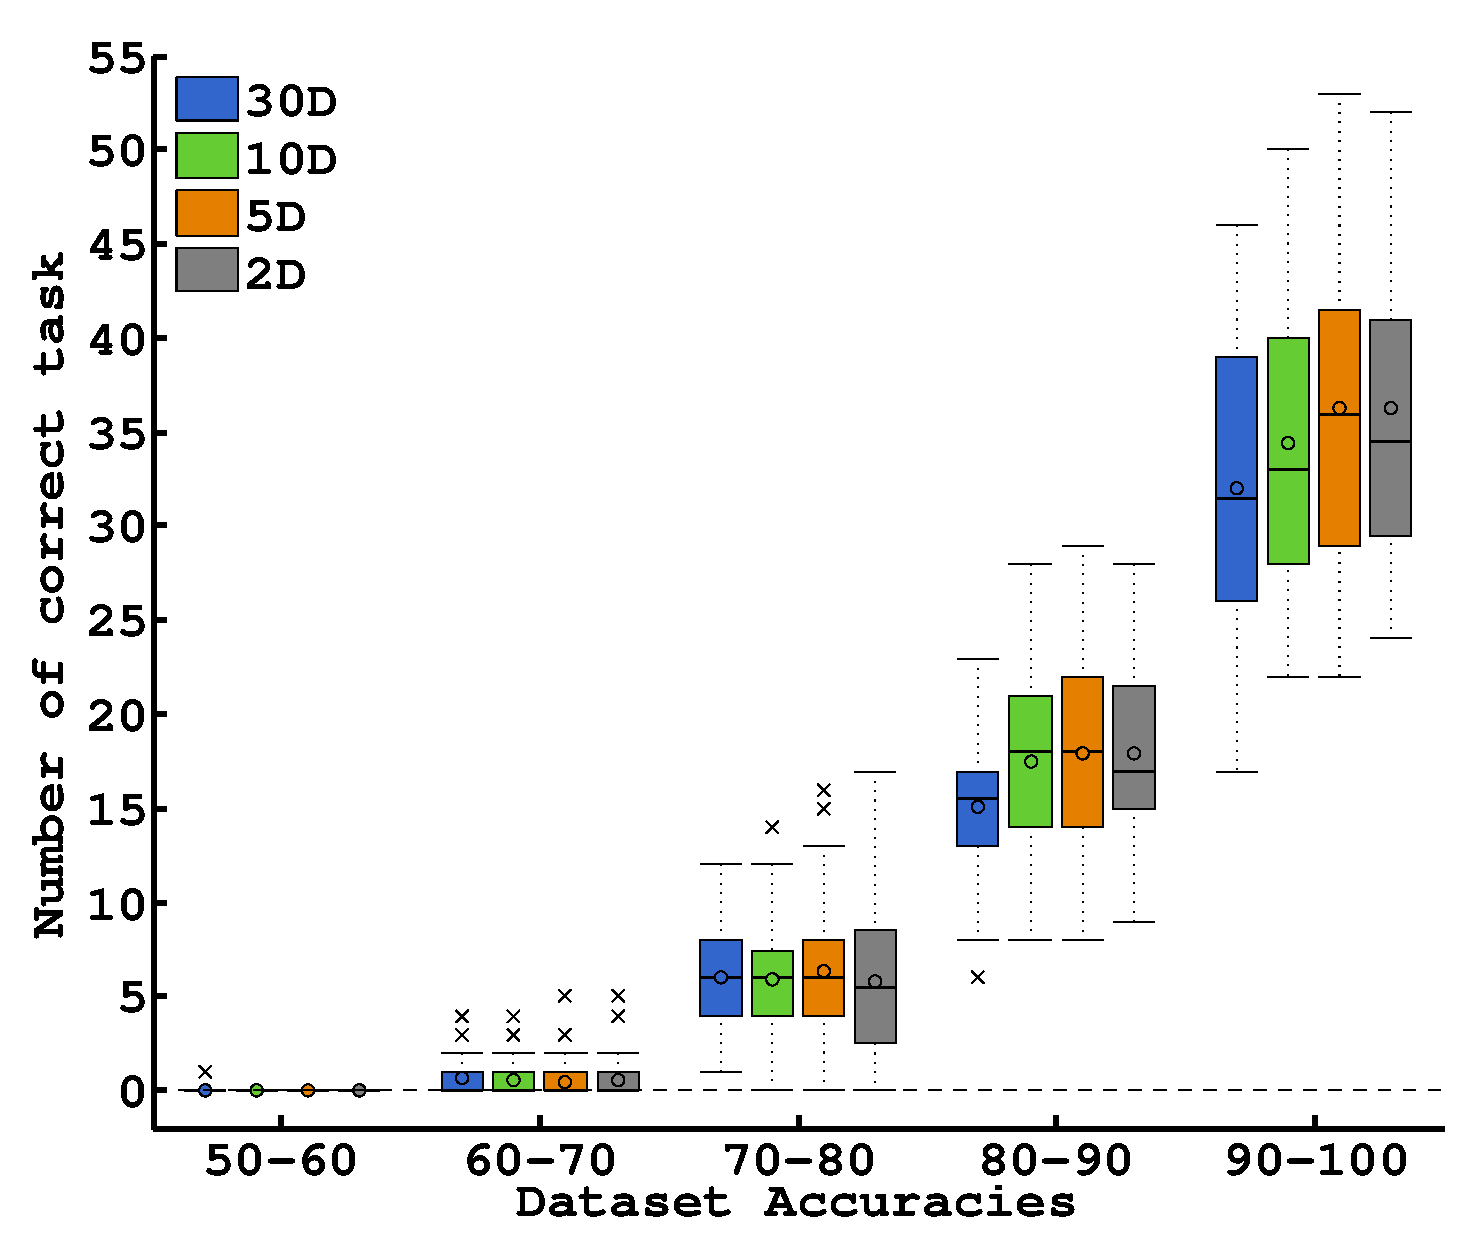
\includegraphics[width=\columnwidth]{img/plots_aaai/plot_artificial_nCorrect.eps}
% 			\caption{Quality of dataset impacts the number of task identified in 500 steps, more evidence should be collected to reach the confidence threshold.}
% 			\label{fig:nCorrectArtificial}
% \end{minipage}
% \end{figure*} 

% \begin{figure}[t]
% \centering
% 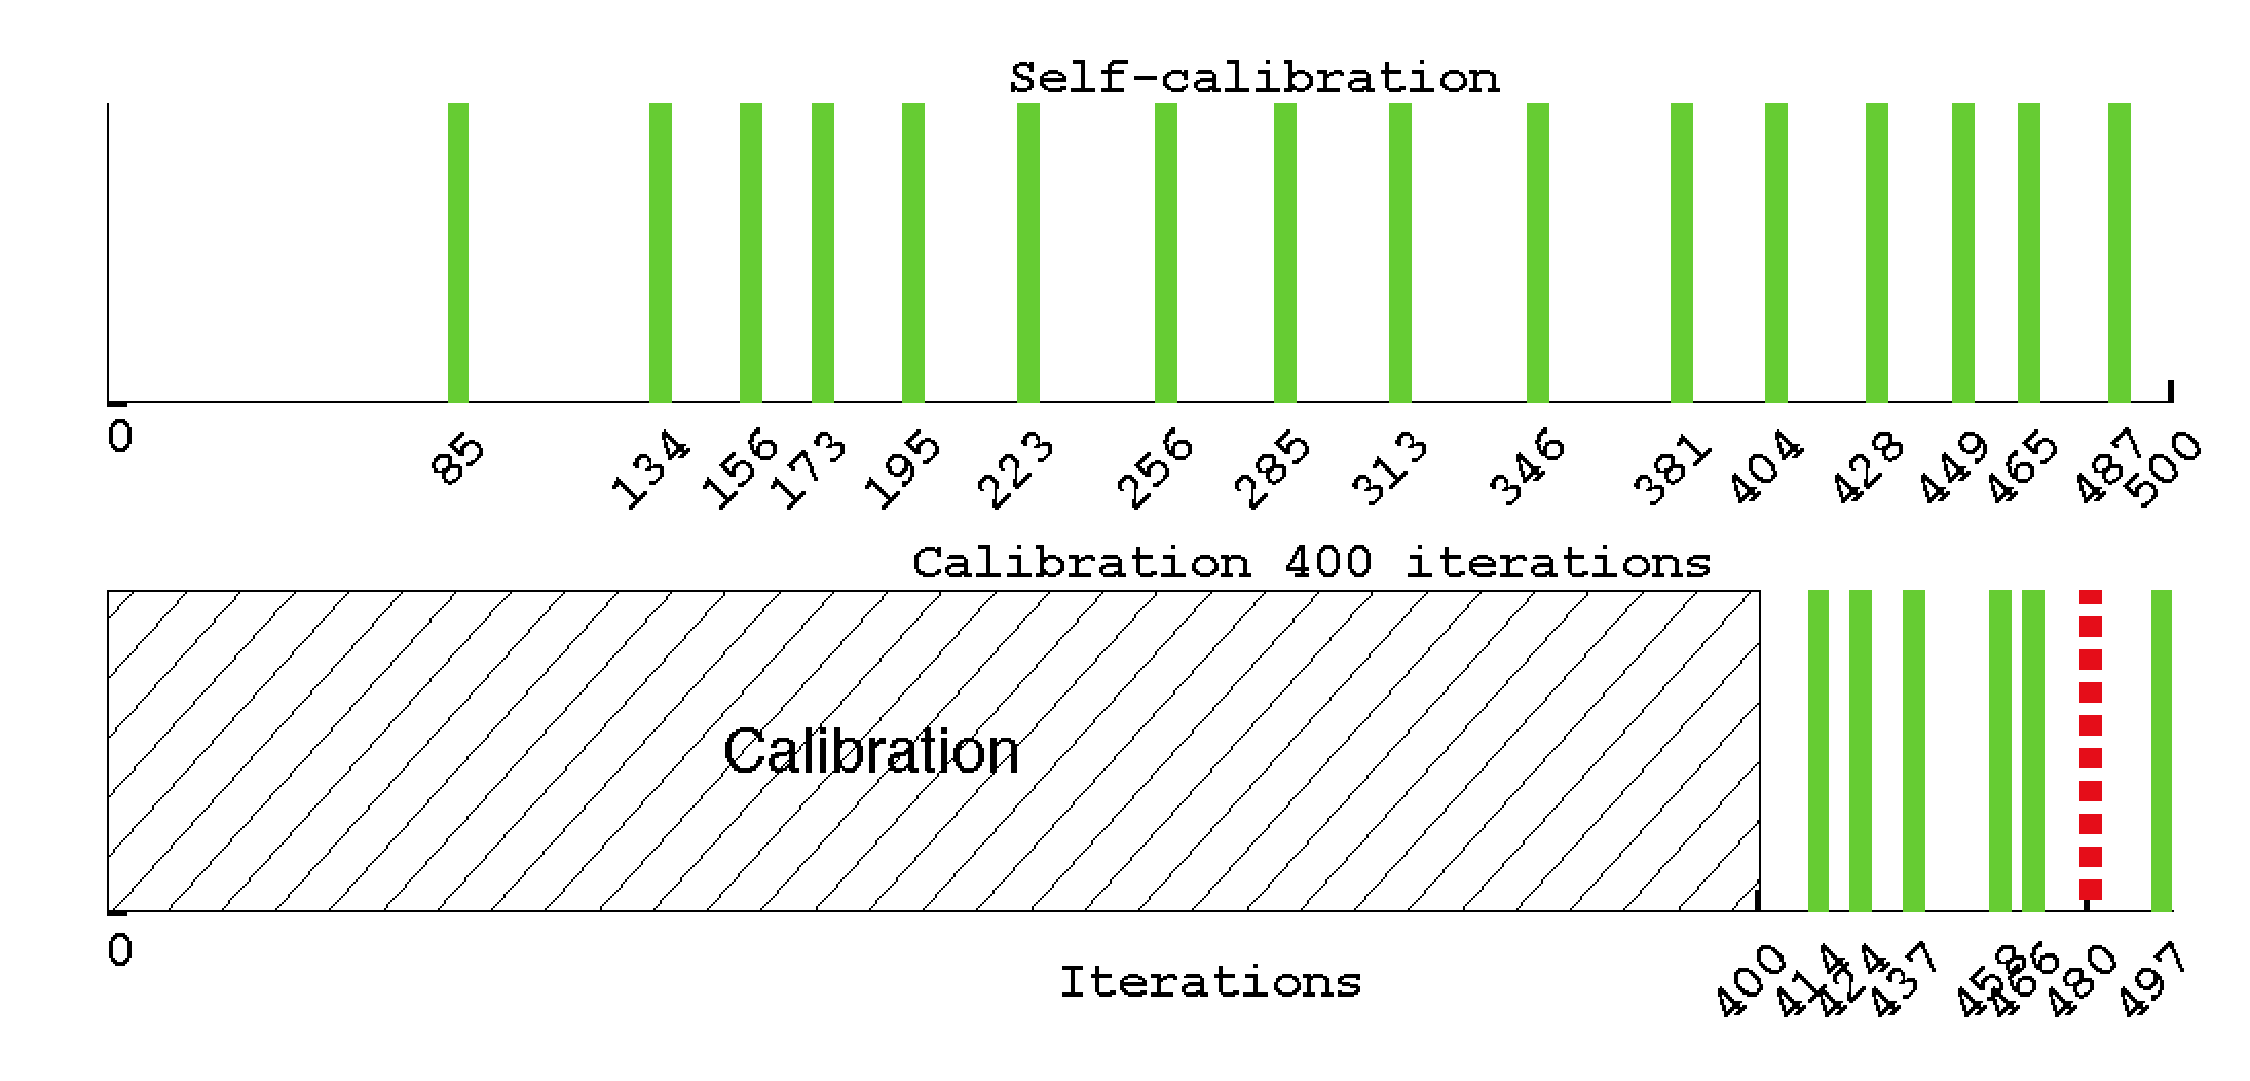
\includegraphics[width=\columnwidth]{img/plots_aaai/plot_the_aaai_sequence.eps}
% \caption{The proposed self-calibration method allow to reach a first task faster, with performance increasing with time. One run from EEG dataset of 83 percent accuracy, self-calibration versus 400 steps calibration.}
% \end{figure} 









%!TEX root = aaai2014.tex
\section{CONCLUSION}
\label{sec:conclusion}


%Discuss the limits (we need to know which model will be able to differentiate the data beforehand therefore we can not test and tune different classifiers, we should not overfit, we should know where to look for), perspectives. Here again first saying that it is interesting to think about this problem. And only then to open to possible application.


In this paper we have shown that, given a limited number of possible tasks, it is possible to solve sequential tasks using human feedback without defining a map between feedback signals and their meaning beforehand. The proposed algorithm optimizes a pseudo-likelihood function and performs active planing according to the uncertainty in the task and meaning spaces. Indeed, taking into account this uncertainty is crucial to solve the task efficiently and to recover the actual meanings. This combination allows: 
\begin{inparaenum}[a)]
\item a human to start interacting with a system without calibration;
\item to automatically adapt calibration time to the user needs which can even outperform fixed calibration procedures; 
\item to adapt to the uncertainty of the information source from scratch.
\end{inparaenum}
We showed the applicability of the approach to brain-machine interfaces based on error potentials which could work out of the box without calibration, a long-desired property of this type of systems.  

%It allows
%\begin{inparaenum}[a)]
%\item a human to start interacting with a system using its own prefered signal
%\item to learn a first task faster and more reliably than with a calibration procedure
%\item to adapt to the uncertainty of the information source from scratch.
%\end{inparaenum}
%%
%%An important assumption of our method is that it is possible to define a finite — and reasonable — set of task hypothesis. This assumption is limiting for many theoretical problems but many useful real word application can still benefit from it Such as the problem of grasping, on a table, one object among a finite set of objects. In this scenario the set of hypothesis consist of all the objects on the table.

%If confirmed on real online experiments, results from EEG datasets demonstrate the real-world application potential of our algorithm. Without the need for calibration, which requires an expert to collect data and train the classifier, BCI technologies may go out of the labs.

% An assumption of the system is that the classifier used is well suited to represent the signals, whereas a calibration procedure allow to test and tune the classifier once the data are acquired.
% Symetrics cases: We note we need to ensure there is at least one action that disambiguate among hypothesis.
A number of open questions remain to be addressed:
\begin{itemize}

\item How the task properties (symmetries, size, \ldots) affect the learning properties?

\item How to leverage from the finite set of hypothesis constraint? A potential avenue is to use a combination of particle filter and regularization on the task space.

% \cite{orsborn2012closed}?
 % phase versus our self-calibration method?

 % \item In invasive BCIs, Orsborn et al. \cite{Orsborn2012} learned to adapt in closed loop a brain decoder. 

\item In real-world applications, users are usually told how to interact with machines. Do people want to have an open-ended choice about what signal to use? Would they be more efficient? When is it better to use a calibration procedure?

\item Only prerecorded datasets have been used. However, signals may change during the learning. For instance, people can try to adapt themselves to a robot if they believe the latter is not understanding properly. Or, brain signals are sensitive to the protocol, the duration of the experiment or even the percentage of errors made by the agent \cite{chavarriaga2010learning}. To which extend the behavior of our agent changes the properties of the teaching signal? Can we adapt to such changes online? 
\end{itemize}

%The work is also relevant with regards to infant social development and learning, as well as in adult mutual adaptation of social cues. This has been the subject of experiments in experimental semiotics \cite{galantucci2009experimental}, such as in the work of Griffiths et al. \cite{griffiths2012bottom} who conducted an experiment with human learners learning the meaning of unknown symbolic teaching signals. An innovative direction would be to embed the algorithmic principles introduced in this paper for experimental linguistics studies.

Finally, while we only considered correct/incorrect labels, in other works we have considered the use of guidance instructions (go up, go left, ...) in human-robot interaction scenario \cite{grizou2013robot}. But increasing the set of possible labels logically requires collecting more examples to obtain a good enough representation of the different signals. Hence, for BCI domains, it is reasonable to keep a limited number of labels.





% \newpage

\section*{Acknowledgments}
We thank the anonymous reviewers for their helpful comments. Work partially supported by INRIA, Conseil R\'egional d'Aquitaine, the 3rd Hand Project (funded under 7th FWP), and the ERC grant EXPLORERS 24007; and from the Spanish Ministry via DPI2011-25892 (L.M.), and DGA-FSE grupo T04.

% The authors from INRIA are with the Flowers Team, a join INRIA - Ensta ParisTech lab, France. Luis Montesano is with Instituto de Investigaci\'{o}n en Ingenier\'{i}a de Sistemas, Universidad de Zaragoza, Spain. I\~{n}aki Iturrate is with the Chair in Non-invasive Brain-Machine Interface (CNBI) and Center for Neuroprosthetics and Institute of Bioengineering, EPFL, Switzerland.

\bibliographystyle{ieeetr}
\bibliography{uai}

\end{document}

